\chapter{Co-located Collaboration with Multi-user Immersive Display}
\label{chapter:colocated_colab}
\minitoc

\section{Introduction}
Immersive CVEs can be used to connect networked users to the same virtual place for collaboration. Users can be both geographically distributed or co-located at the same physical place. Compared to remote situations, co-located users share the same physical workspace which allows direct user communication and interaction without computer mediation, and unlike cases in which co-located users collaborate with 2D graphic user interface (e.g. image wall, interactive table), immersive CVEs allow them to share the same virtual world on top of the same real space.

A major problem of using immersive CVE for co-located collaboration is that classical projection-based immersive displays can only show images generated from a single user's viewpoint and others sharing the same images from another location will suffer visual distortion. To tackle this problem, multi-user immersive displays are designed to offer individual stereoscopic views for multiple users.

This chapter concentrates on how co-located users collaborate inside multi-user immersive virtual environment and it is divided into two sections. The first presents technical aspects related to multi-user immersive displays and summarizes existing methods to separate images for different users. The second describes notions that allow us to define two collaborative modes that form a general framework for co-located collaboration, and then presents two major issues that we identify during the collaboration process and proposes research methodology that we adopted to solve the aforementioned issues.  


\section{Multi-user Immersive Display}
Immersive display constitutes a main component of immersive virtual environment as the visual sense plays a predominant role in user's perception process. As mentioned in previous chapter (section~\ref{sec:visual_interface}), immersive displays differ from traditional displays in that they have large field of view, high resolution, stereoscopic images associated with viewpoint tracking technology.


\subsection{Stereoscopy}
\label{sec:stereo}

Stereoscopy is the production of the illusion of depth by presenting a pair of 2D images showing two perspectives that both eyes naturally have in binocular vision. Then the brain merges the two images into a ``single" one to achieve stereopsis \citep{Blake2006Perception}. Besides stereoscopy, other cues (e.g. object occlusion, linear perspective, etc.) can also help to determine relative distances and depth in a perceived scene, but stereoscopy remains the most effective factor that provides users with instant depth perception.

To achieve stereoscopic vision, we should first generate a pair of images depending on user's head position and orientation, as well as the interpupillary distance (IPD) \citep{Dodgson2004IPD}. Then we need to provide two images separately for each eye. Existing separation methods can be classified into three categories:

\begin{itemize}
\item Head-mounted displays: we can put two small screens in front of the eyes, or a single screen displaying two images side by side to show only the desired image to each eye (Figure~\ref{fig:1_vi:hmd});
\item Auto-stereoscopic screen: auto-stereoscopic display separate images at the screen level by using the lenticular lenses or parallax barrier to assure that each eye of the user sees different pixel columns which correspond to two different images \citep{Perlin2000Autostereo};
\item Eyeglasses separation: images can be separated passively by colorimetric differentiation or polarized glasses, or actively by rapidly alternating shuttered glasses.
\end{itemize}

Each type of stereoscopic display has its advantages and inconveniences. HMD is the most straightforward way to provide two different images for the eyes and allows fully visual immersion of the user (the real world is completely blocked from user's eyes except for see-through HMDs \citep{Schmalstieg2002Stube}). However, various technical limitations like limited resolution and field of view enhance user's visual fatigue and restrain the wide use of HMDs. Unlike HMDs that are heavy to carry, eyeglasses based technology combined with large immersive projection display (e.g. image wall, CAVE, dome) gives user a more comfortable stereo experience. Auto-stereoscopic screens do not require user to equip any glasses or headgear, but have limited work range - user should stay at predefined position (at a certain distance from the screen) to correctly perceive stereo images.

Recent technical developments largely improved the usability of all three types of stereoscopic display. HMDs now are lighter and less expensive with more compact design, along with better resolution, larger field of view. The improvements of immersive projection technology (IPT) \citep{Bullinger1997Immersive} makes projection-based systems with eyeglasses a widespread solution both in academic institutes and industries, and they are specially useful to create large immersive virtual environment for group immersion by the combination of multiple projectors, such as CAVEs. Auto-stereoscopic screen combined with user tracking can now allow the tracked user to pass through different viewing areas without discontinuity \citep{Kooima2010Tiled}, but still requires complex hardware and software setup. So HMDs and projection-based systems become the major platform to support immersive or partially-immersive experience.


\subsection{Visual Distortion}
Stereoscopic images are generated from a single location - the center of projection (CoP) \citep{Banks2009Perception}. A user can properly perceive the displayed 3D content on a projection screen when viewed from the CoP. So in an immersive virtual environment, user's viewpoint is captured by head-tracking to serve as the CoP to generate appropriate images in real time as the user moves physically.

While HMDs provide personal stereoscopic images for a single user, projection-based systems are often shared by a group of people for team work, as shown by Figure~\ref{fig:2_group}. In such multi-user situation, only the tracked user receives correct stereo images from the CoP, other co-located users (followers) share the same stereo images intended for the tracked user and participate passively in the collaborative task \citep{Bayon2006Multiple}. When users are close enough to the tracked user, they can get a relatively faithful representation of the virtual environment, but as the distance increases, displacement from the CoP results in increasingly inappropriate stereo cues and distorted perception of the virtual space.

\begin{figure}[htb]
  \centering
  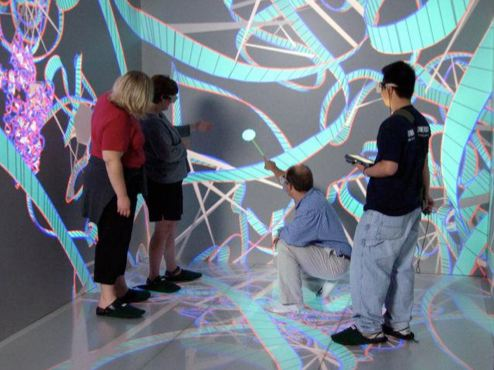
\includegraphics[width=0.6\textwidth]{figures/ch2/group}
  \caption{\label{fig:2_group}A group of people collaborating in a CAVE for data visualization \citep{Pollock2012Right}.}
\end{figure}

\begin{figure}[htb]
  \centering
  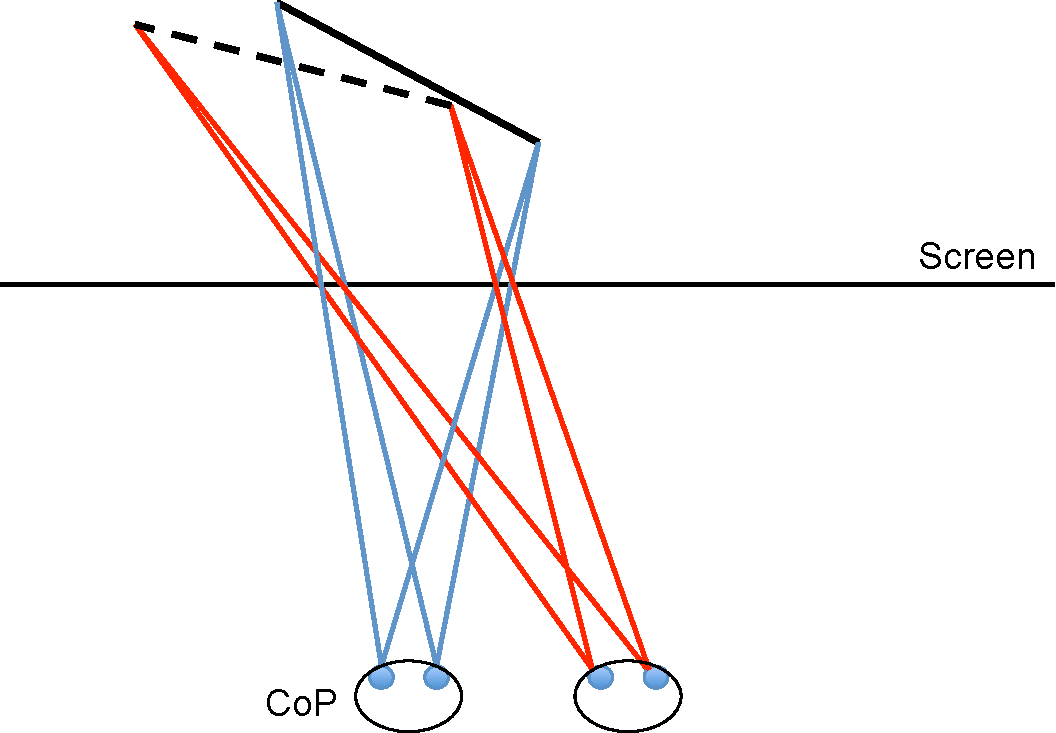
\includegraphics[width=0.48\textwidth]{figures/ch2/distortion_1}
  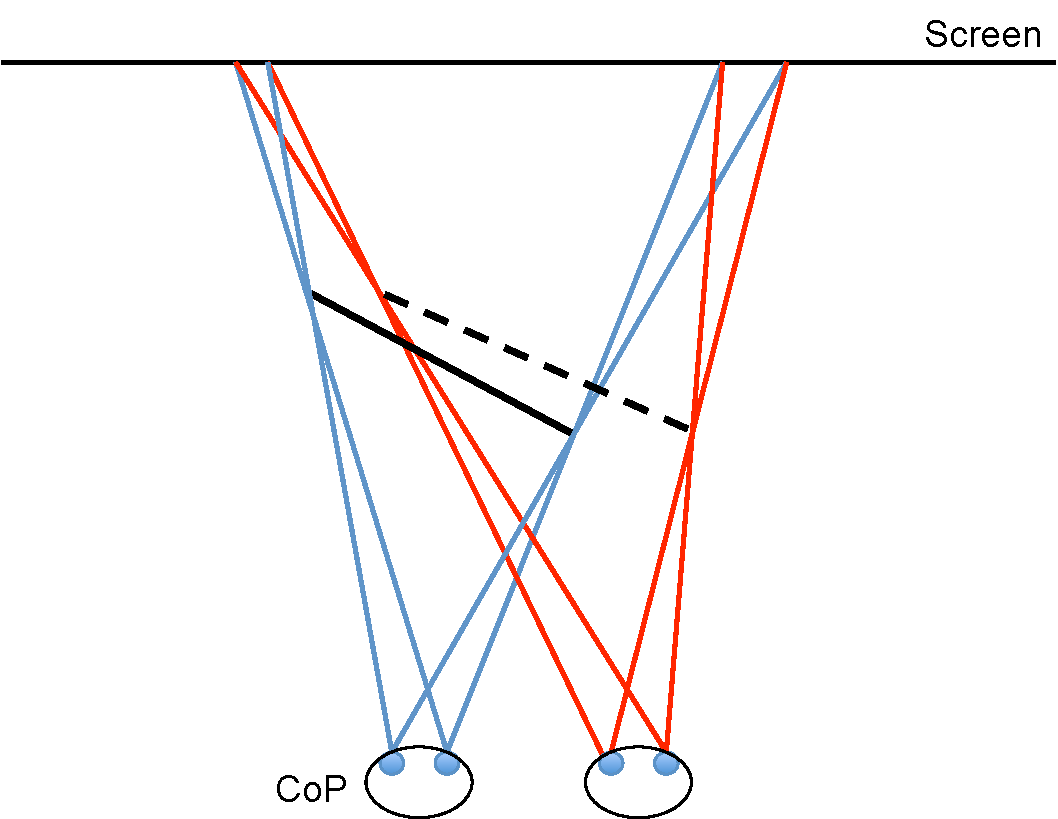
\includegraphics[width=0.48\textwidth]{figures/ch2/distortion_2}
  \caption{\label{fig:2_ray_model}Illustration of visual distortion by perceiving the right view from a location other than the CoP. The black line represents the correct view of object perceived from CoP and the dotted line corresponds the distorted view observed from another location.}
\end{figure}


Visual distortion caused by displacement from the CoP can be predicted by a ray-intersection model \citep{Burton2012Diagnosing}. As shown by Figure~\ref{fig:2_ray_model}, no matter the virtual object is situated behind or in front of the screen, a lateral displacement from the CoP will cause deformation and shift of the perceived object. Similar effects can be observed by moving forward or backward with respect to the CoP.

A series of studies have been conducted to assess the influences of such visual distortion. When viewing monocular displays from locations displaced from the CoP, the spatial judgments remain relatively acceptable. \citet{Vishwanath2005Pictures} investigated the mechanism underlying this perceptual invariance by studying the perceived shapes of pictured objects viewed from various locations and they find that invariance is achieved through the awareness of the 2D picture plane. However, when it comes to stereo images, \citet{Banks2009Perception}'s experiment indicates that human viewers of stereo pictures are unable to compensate for incorrect viewing position. This result is confirmed by follow-up studies: judgments of angles are distorted after leftward and rightward displacement from the CoP \citep{Burton2012Diagnosing} and judgments of object depth are distorted after forward and backward displacement from the CoP \citep{Pollock2012Right}, although the magnitude of these distortions is consistently less than predicted by the ray-intersection models. More studies on visual distortions in stereoscopic systems can be found in articles by \citet{Woods1993Image, Held2008Misperceptions, Ponto2013Perceptual}.


\subsection{View Separation}
To better support co-located use of immersive virtual environments, we need to provide perspective-correct (distortion free) individual stereoscopic views for each user. One direct way is to use personal displays such as HMDs \citep{Salzmann2008TUS} or see-through HMDs \citep{Schmalstieg2002Stube}, and another solution is to introduce adaptations to existing immersive displays which already support group immersion.

\citet{Bolas2004New} categorize solutions for displaying multiple images in a common area:

\begin{itemize}
\item Spatial barriers use the display's physical configuration and user placement to block users from seeing each other's view.
\item Optical filtering involves systems that filter viewpoints using light's electromagnetic properties, such as polarization or wavelength.
\item Optical routing uses the angle-sensitive optical characteristics of certain materials to direct or occlude images based on the user's position.
\item Time multiplexing solutions use time-sequenced light and shutters to determine which user sees an image at a given point in time.
\end{itemize}

Except the first solution, the three other options are the same technologies that are used to separate images for the left and right eye of a single user as presented in section~\ref{sec:stereo}. Multi-user systems are often build with mixed solutions from these categories, here is a description of existing systems that provide independent stereo images for different users inside immersive or semi-immersive environment.


\subsubsection{Image Separation} 
Typically we can create separate image channels for different users by adding shutters and/or optical filters in front of projectors combined with synchronized counterparts in front of user's eyes.

The two-user Responsive Workbench developed by \citet{Agrawala1997TRW} relies purely on a time-multiplexing method which displays four different images in sequence on a CRT projector at 144Hz, thus each eye of a user views the virtual scene at 36Hz (Figure~\ref{fig:2_sep_active:wb}). This workbench is the first demonstration of a two-user stereoscopic system, but the time-multiplexing method largely reduces projection time for each eye (low brightness) and users suffer from image flicker and crosstalk. \citet{Blom2002Multiple} then extended this active shuttering method to multi-screen systems like CAVEs. \citep{Froehlich2004Implementing} further studied active shuttering technology by testing two kinds of shutters on the projector side with a range of shuttering frequencies (Figure~\ref{fig:2_sep_active:four}). The mechanical shuttering delivers higher brightness and less cross talk, but does not extend as easily to more than two users as liquid crystal (LC) shutters because of the required rotation speed and size of the disc. They tested LC shutters from 140Hz to 400Hz and found that users did not perceive flicker above a refresh rate of 200Hz, but a frequency higher than 320Hz would result in very dark images.

\begin{figure}[htb]
  \begin{subfigure}{.5\textwidth}
    \centering
    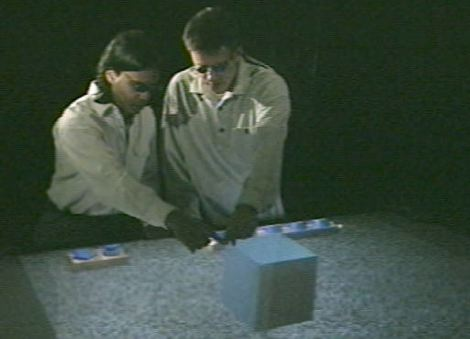
\includegraphics[height=5cm]{figures/ch2/resp_workbench}
    \caption{The two-user Responsive Workbench.}
    \label{fig:2_sep_active:wb}
  \end{subfigure}
  \begin{subfigure}{.5\textwidth}
    \centering
    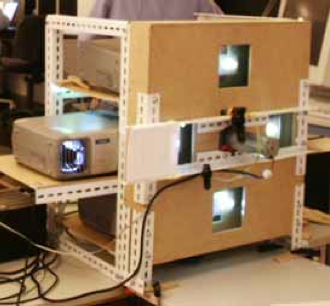
\includegraphics[height=5cm]{figures/ch2/four_proj}
    \caption{Two-user active separation with four projectors.}
    \label{fig:2_sep_active:four}
  \end{subfigure}
  \caption{\label{fig:2_sep_active}User separation by time-multiplexing with active shutters.}
\end{figure}

\begin{figure}[htb]
  \begin{subfigure}{.5\textwidth}
    \centering
    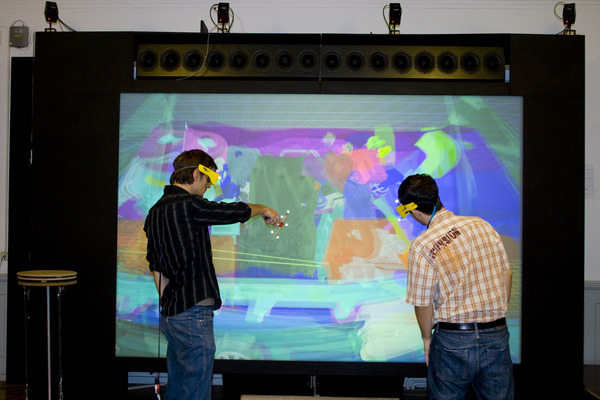
\includegraphics[width=\linewidth]{figures/ch2/multiview_wall}
    \caption{Wall display for two users.}
    \label{fig:2_sep_active_passive:wall}
  \end{subfigure}
  \begin{subfigure}{.5\textwidth}
    \centering
    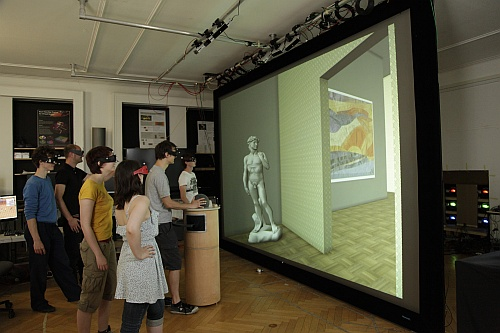
\includegraphics[width=\linewidth]{figures/ch2/C1x6}
    \caption{The six-user projection wall display.}
    \label{fig:2_sep_active_passive:6user}
  \end{subfigure}
  \caption{\label{fig:2_sep_active_passive}User separation by active time-multiplexing combined with polarization.}
\end{figure}

Another solution is to combine time-multiplexing with polarization filters. In 1999, Barco developed the ``Virtual Surgery Table"\footnote{http://www.barco.com/en/Products/Compact-Multi-User-Projection-Table.aspx/} which provides two users with stereoscopic images by differently polarizing the output of two active stereo projectors. Then \citet{Frohlich2005MultiViewer} extended this shuttered display to support up to four users with eight shuttered liquid-crystal display (LCD) projectors (Figure~\ref{fig:2_sep_active_passive:wall}). In this setup, images for different users are separated by active shutter glasses while the separation of the images for the left and right eye is ensured by passive polarized filters. This approach shows better performance in terms of perceived flicker, brightness of each view and crosstalk compared to purely active shuttering method.


\citet{Frohlich2005MultiViewer} also summarized three main parameters can be considered to evaluate the quality of a multi-stereoscopic projection system:

\begin{itemize}
\item Brightness per view;
\item Static and dynamic crosstalk; 
\item Perceived flicker, which depends on the shutter frequency, the video rate of the projector and brightness.
\end{itemize}

In 2011, \citet{Kulik2011CSS} developed a projection-based stereoscopic display for six users by using six customized digital light processing (DLP) projectors running at 360Hz for a single screen, which results in 60Hz per user (Figure~\ref{fig:2_sep_active_passive:6user}).


\citet{Dodgson2005Autostereoscopic} provided an introduction and overview of auto-stereoscopic multi-view displays. Users in this kind of multi-view system get perceive 3D objects from his/her own point of view without tracking or eyeglasses, but only inside a limited zone depending on different properties of the display. Another issue is that with increasing number of views (e.g. up to 256 views by \citet{Takaki2010Multi}), generating images in real time for dynamic interaction would be a challenge.

\subsubsection{Spatial Separation}
Instead of creating image channels, we can also take advantage of the spatial property of the display by assigning different screens or parts of a single screen to different users. For example, the ``Protein Interactive Theater" (PIT) \citep{Arthur1998PIT} uses two orthogonal screens and each user looks at only one of the screens (Figure~\ref{fig:2_sep_spatial:pit}). The IllusionHole \citep{Kitamura2001Interactive} uses a circular mask on top of a tabletop projection. By looking through the mask, users positioned around the table see their individual stereo images shown in different areas of the screen (Figure~\ref{fig:2_sep_spatial:illu}). Other systems like the Virtual Showcase \citep{Bimber2006Virtual}and Joint Space Station \citep{Mulder2004Modular} use similar mirror-based display to support multiple users. These desktop-based systems are often designed to accomplish specific collaborative tasks (e.g. 3D object visualization) and provide limited workspace with inherent spatial constrains. 

\begin{figure}[htb]
  \begin{subfigure}{.45\textwidth}
    \centering
    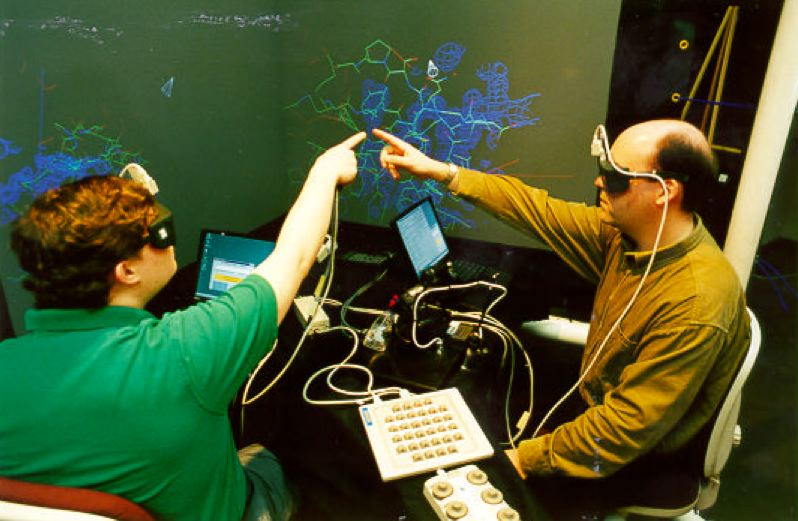
\includegraphics[height=4.5cm]{figures/ch2/pit}
    \caption{The PIT system for two-user collaboration.}
    \label{fig:2_sep_spatial:pit}
  \end{subfigure}
  \begin{subfigure}{.55\textwidth}
    \centering
    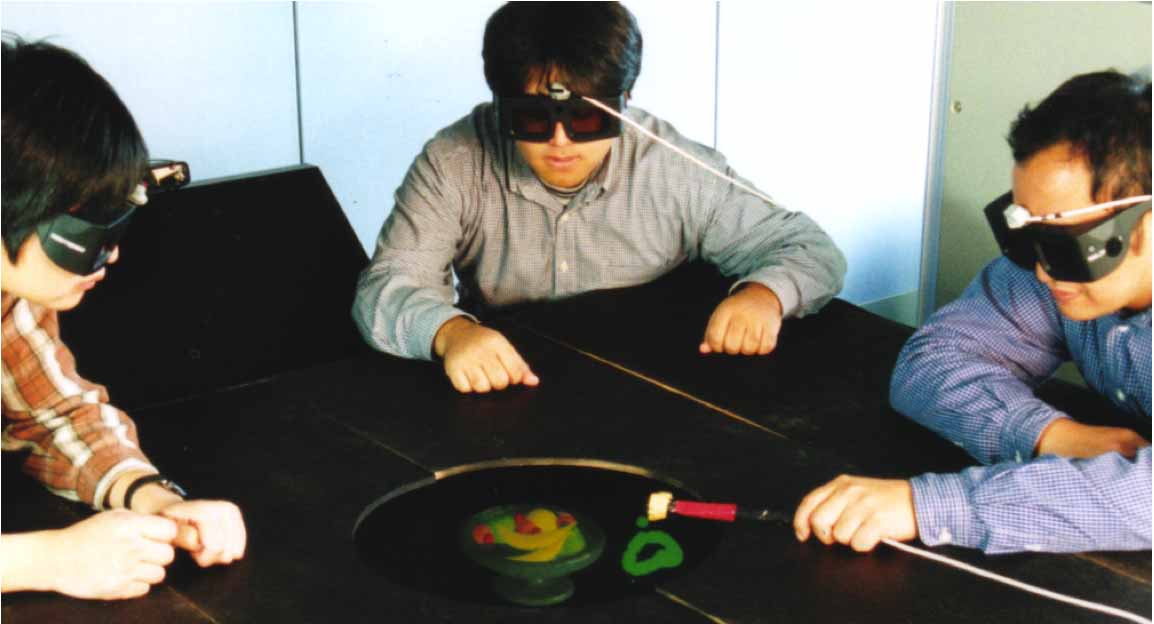
\includegraphics[height=4.5cm]{figures/ch2/illusionHole}
    \caption{The IllusionHole for tabletop collaboration.}
    \label{fig:2_sep_spatial:illu}
  \end{subfigure}
  \caption{\label{fig:2_sep_spatial}User separation by using different screens or different parts of the same screen.}
\end{figure}

When using larger wall display or CAVE, users can have head-tracked individual monoscopic \citep{Maksakov2010Whale} or stereoscopic views \citep{Schulze2012Democratizing} on different parts of the display. When they share the same part of the screen, sophisticated algorithms are applied to recalculates images based on an averaged viewpoint depending on positions and orientations of all tracked users. These software-based solutions allow co-located collaboration in immersive virtual environment without additional hardware setup, although the reduced visual distortions could still be disturbing for certain tasks that require precise spatial operations (e.g. object co-manipulation).

\subsubsection{Other Methods}
There are also many other display solutions offering individual stereoscopic views like the volumetric display \citep{Grossman2008Volum} and holographic display \citep{Lucente1997Holo}. However, for now it is still difficult to extend these displays to provide large-scale visual immersion. 

Another interesting multi-user display is the omni-stereo display \citep{Simon2004Omni} such as AVIE \citep{Mcginity2007Avie} and i-Cone \citep{Simon2002Icone} which provides good support for immersive visualization with large user group, but theoretically users need to stay at predefined positions to get good perspective. \citet{Simon2007MVI} compared usability and interaction performance between multi-viewpoint images and head-tracked stereo display. Results showed that for certain tasks that users do not need to move physically (e.g. ray-casting selection and in-hand object manipulation), multi-viewpoint images can produce similar or even better performance than fully head-tracked interaction.


\subsection{Summary}
This section gives a general presentation of multi-user immersive display from the initial motivation (to provide distortion-free stereoscopic view for each user) to various implementations.

Among all presented multi-user display technologies, the active \& passive method which combines time-multiplexing with polarization filters is the most effective and cost-efficient way to build multi-user immersive virtual environment. There are multiple reasons: first, it completely eliminated visual distortion due to observation from another position than the CoP; second,
it can be easily applied to different shapes of large-scale immersive systems like walls, CAVEs or domes without imposing strong spatial constrains on user's position and orientation with respect to the screen(s), users can move inside a relatively large physical workspace; at last, compared to purely time-multiplexing separation, it provides high brightness, low crosstalk and less flicker stereo images.   

% -------------------------------------------------------------------------------------------------


\section{Co-located Collaboration}
When several users work in a multi-user immersive virtual environment for collaborative tasks, they share a virtual world on top of the same physical workspace. This physical collocation forms a mixed context which lies in the middle of \citet{Milgram1995AR}'s reality-virtuality continuum where user can have direct as well as computer-mediated interaction and communication. While lots of research works focus on supporting remote users to work efficiently together via immersive CVEs, co-located collaboration in the same immersive virtual environment for now receives limited attention. This is mainly due to the rareness and relatively high-cost of multi-user immersive systems, in contrast to non-immersive multi-user systems such as interactive walls and tables that are already widely studied in the CSCW community \citep{Scott2003System, Inkpen2005Exploring}.

Here we focus on co-located collaboration in immersive multi-user systems. Given the characteristics of collaborative work presented in chapter~\ref{chapter:context}, we are mainly interested in following research questions:

\begin{itemize}
\item How users perceive each other and achieve a shared context for collaboration?
\item How to intelligently manage users' viewpoints to support various types of collaborative tasks that require different spatial configuration of users in the virtual world (side-by-side or far away from each other)?
\item How to manage each user's workspace and spatial relationship with other users?
\item How to allow fluent transition between shared and individual activities for each user?
\end{itemize}

Below we begin by presenting different concepts related to spatial arrangement of users in the common physical workspace and the management of their points of view in the virtual world. Then we talk about issues that we identified during collaborative tasks and research methods that are applied to study aforementioned issues.

\begin{figure}[htb]
  \centering
  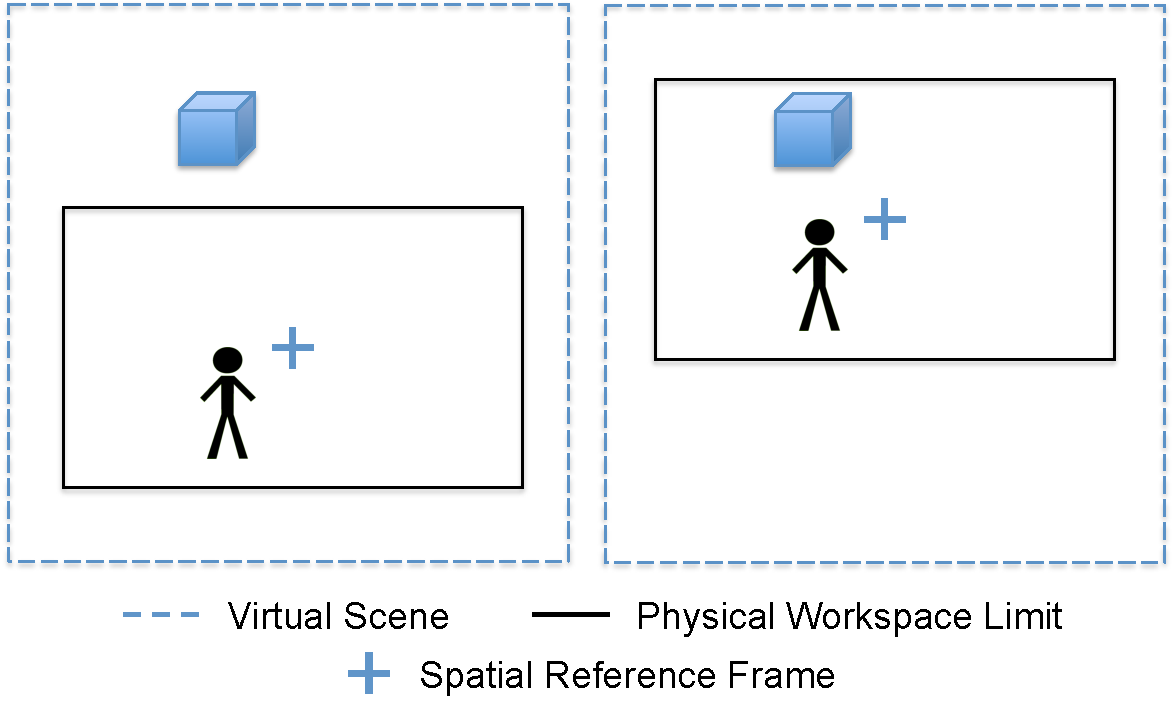
\includegraphics[width=.8\textwidth]{figures/ch2/referenceframe}
  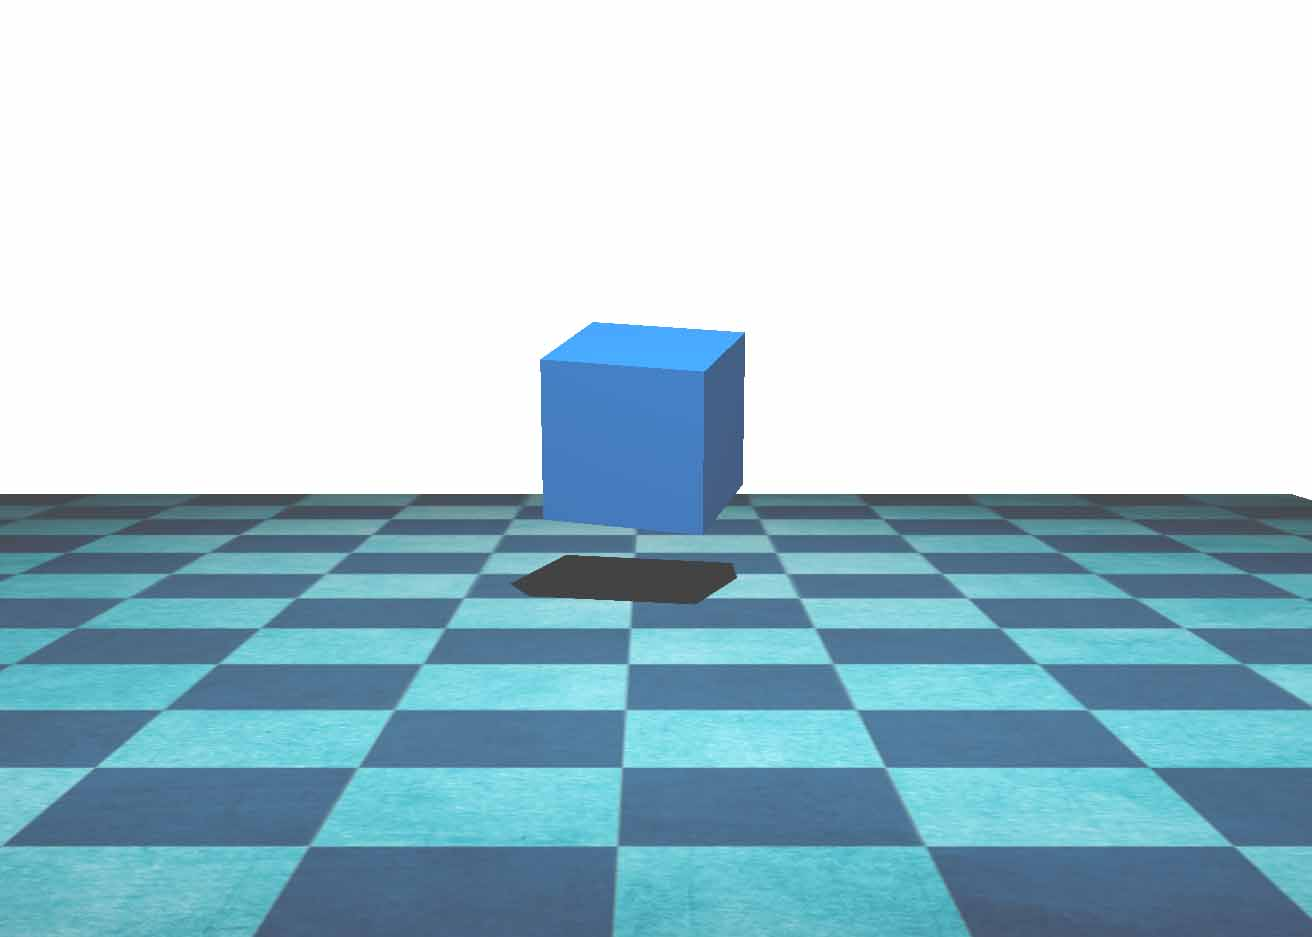
\includegraphics[width=0.48\textwidth]{figures/ch2/ref_1}
  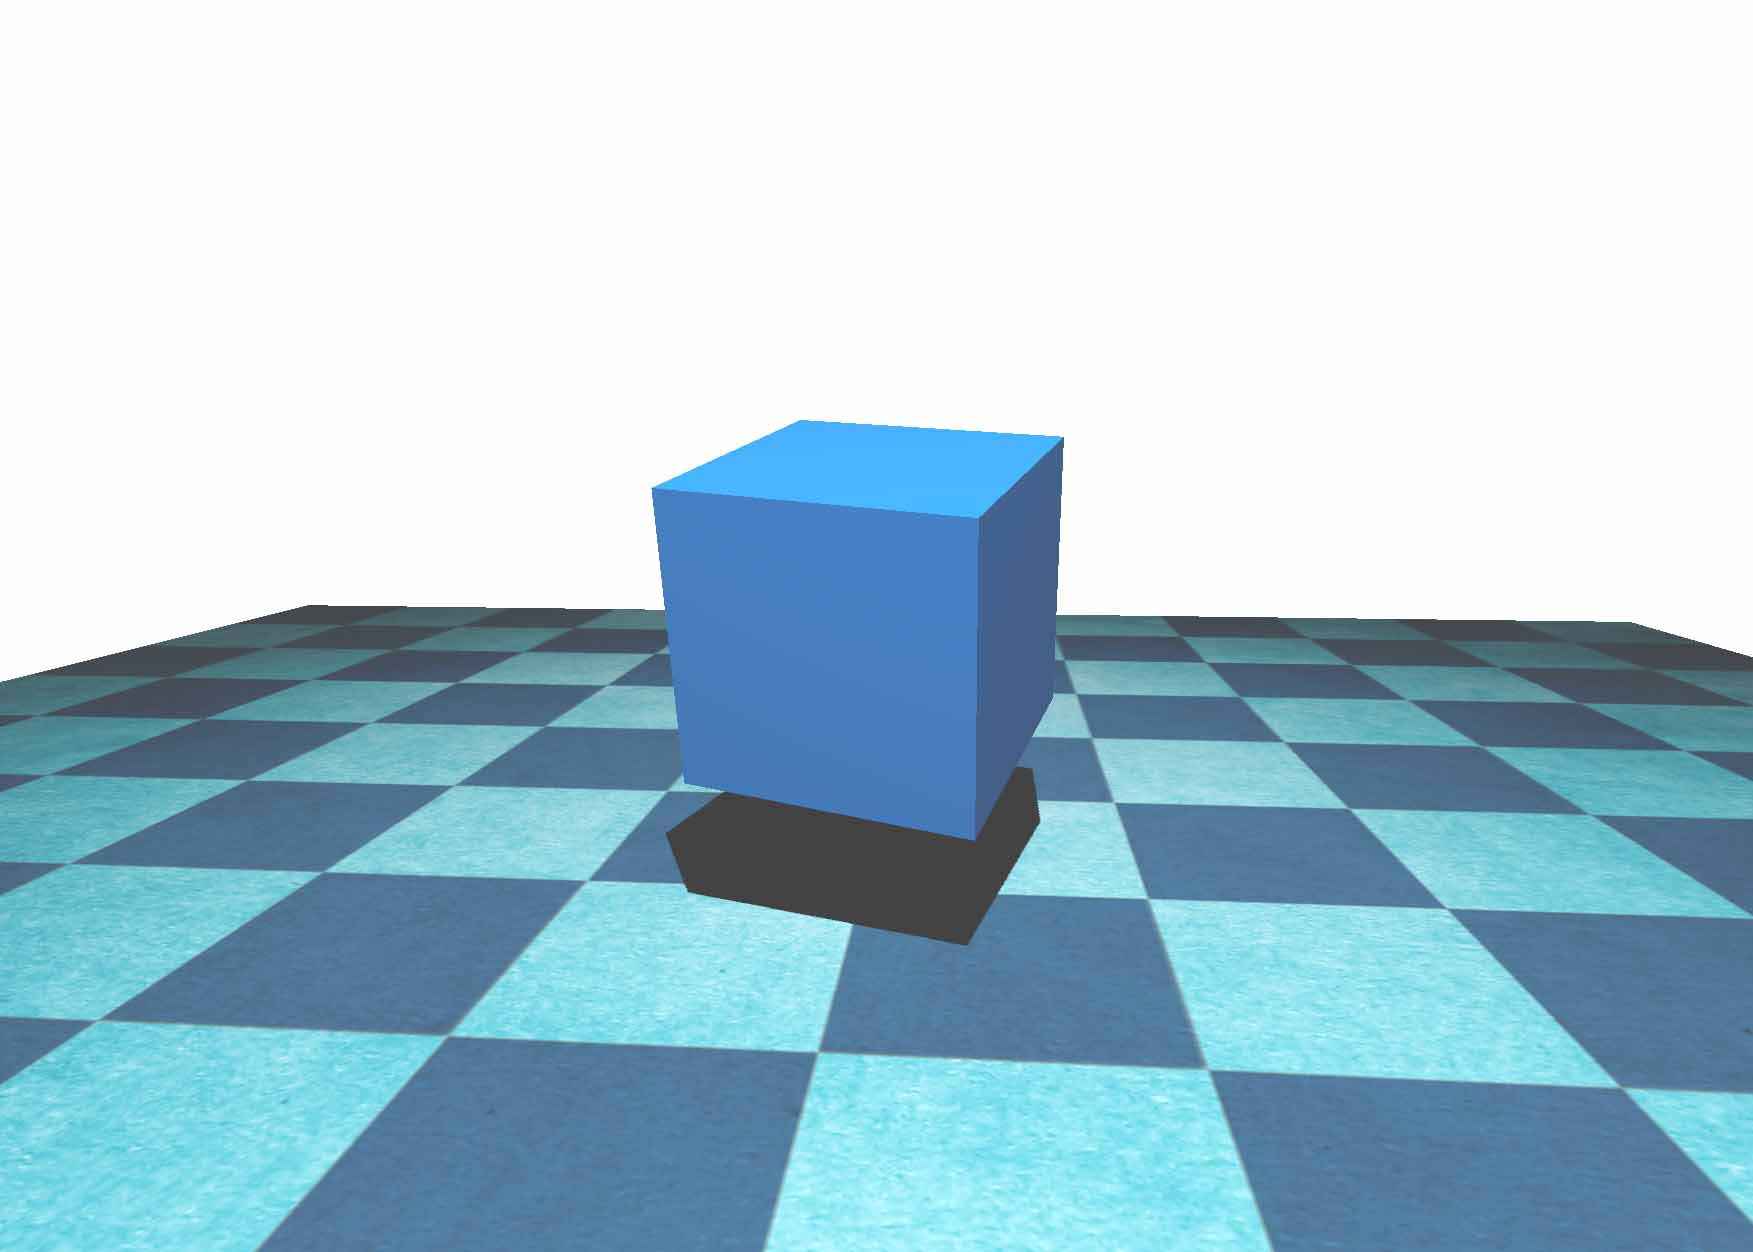
\includegraphics[width=0.48\textwidth]{figures/ch2/ref_2}
  \caption{\label{fig:2_reference}Illustration of the impact of moving spatial reference frame on user's viewpoint location in the virtual scene.}
\end{figure}

\begin{figure}[htb]
  \centering
  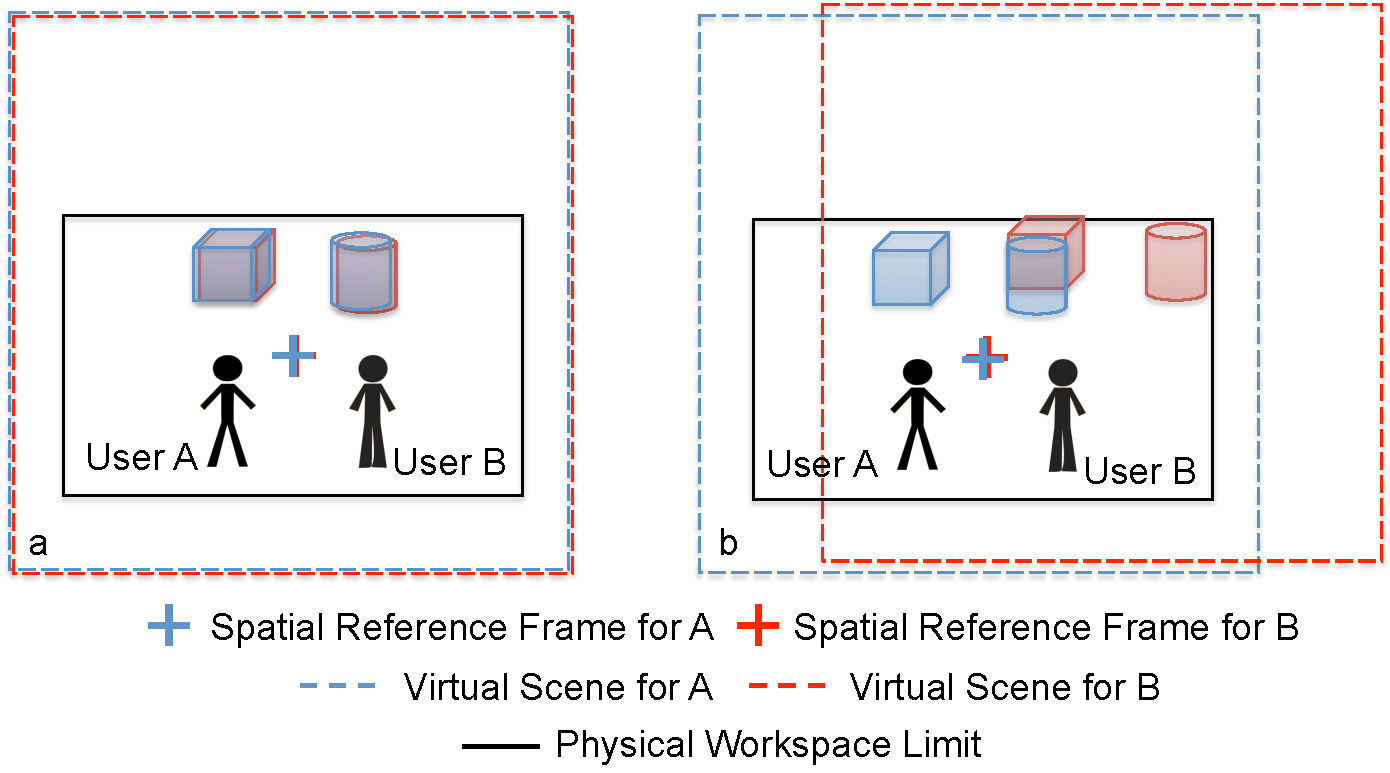
\includegraphics[width=.9\textwidth]{figures/ch2/consistency}
  \caption{\label{fig:2_consistency}Distribution of users' spatial reference frames: a) consistent mode; b) individual mode.}
\end{figure} 

\subsection{Concepts}
\subsubsection{Spatial Reference Frame}
In most VR systems, there is a spatial reference frame that maps user's physical position in the tracking space to a corresponding value in the virtual world, so that the computer can use this position to render proper images corresponding user's point of view. In practice, the spatial reference frame is often expressed as the virtual coordinates of the center of physical workspace defined by the screen and/or tracking device configuration. For example in Figure~\ref{fig:2_reference}, from left to right, user remains at the same position in the physical workspace while the spatial reference frame is set to different location in the virtual world, the user will have different virtual viewpoints accordingly.


\subsubsection{Spatial Consistency}
In a multi-user virtual environment, each user has a corresponding spatial reference frame. The multi-user display system is able to render completely different stereoscopic images for each user depending on the configuration of users' spatial reference frames.

When all reference frames are strictly superimposed, the spatial relationship between users in the virtual world will be consistent with their relative spatial distribution in the real workspace. In an immersive multi-user virtual environment, this spatial consistency allows users to perceive a virtual object at exactly the same physical location from corresponding viewpoints (Figure~\ref{fig:2_consistency}a). This particular situation is quite similar to cases when users collaborate around physical objects in the real world.

Otherwise, each user will no longer perceive the same object at the same physical location. What a user perceives totally depends on the configuration of spatial reference frame in the virtual world. For example in Figure~\ref{fig:2_consistency}b, user B's spatial reference frame is shifted to the left regarding the one of user A, so user B sees a cube in front of him/her while user A considers the same cube to be on user B's left.


\subsubsection{Collaborative Mode}
The distribution of spatial reference frames has a direct influence on how users interact and communicate with each other, so collaboration in multi-user immersive virtual environment can be divided into two modes depending on whether the spatial consistency is maintained among all the users.


\paragraph{Consistent Mode}
In this mode, all users' virtual spaces are consistent with the common physical workspace which result in a shared spatial understanding of the virtual environment. In this context, users can communicate spatial information similarly as in the real world. For example, one can speak to another ``Pass me the book on your left", or point to objects or directions by deictic gestures \citep{Salzmann2009VRPointing} (Figure~\ref{fig:2_consistent_collab:pointing}). Another advantage of consistent mode is that users can make use of tangible devices (props) to get passive tactile feedback for object co-manipulation \citep{Aguerreche2009Three, Salzmann2009CIC} (Figure~\ref{fig:2_consistent_collab:tangible}) or for other specific tasks like two-user driving test \citep{Salzmann2008TUS}, etc.

In projection-based immersive system, we can consider that users' physical bodies are directly ``integrated" into the virtual environment. Social cues that facilitate human communication (e.g. gestures, postures, facial expressions and gaze direction, etc.) can be conveyed without computer mediation. This is a big advantage compared to remote situations where users communicate through embodied avatars. 

\begin{figure}[htb]
  \begin{subfigure}{.3\textwidth}
    \centering
    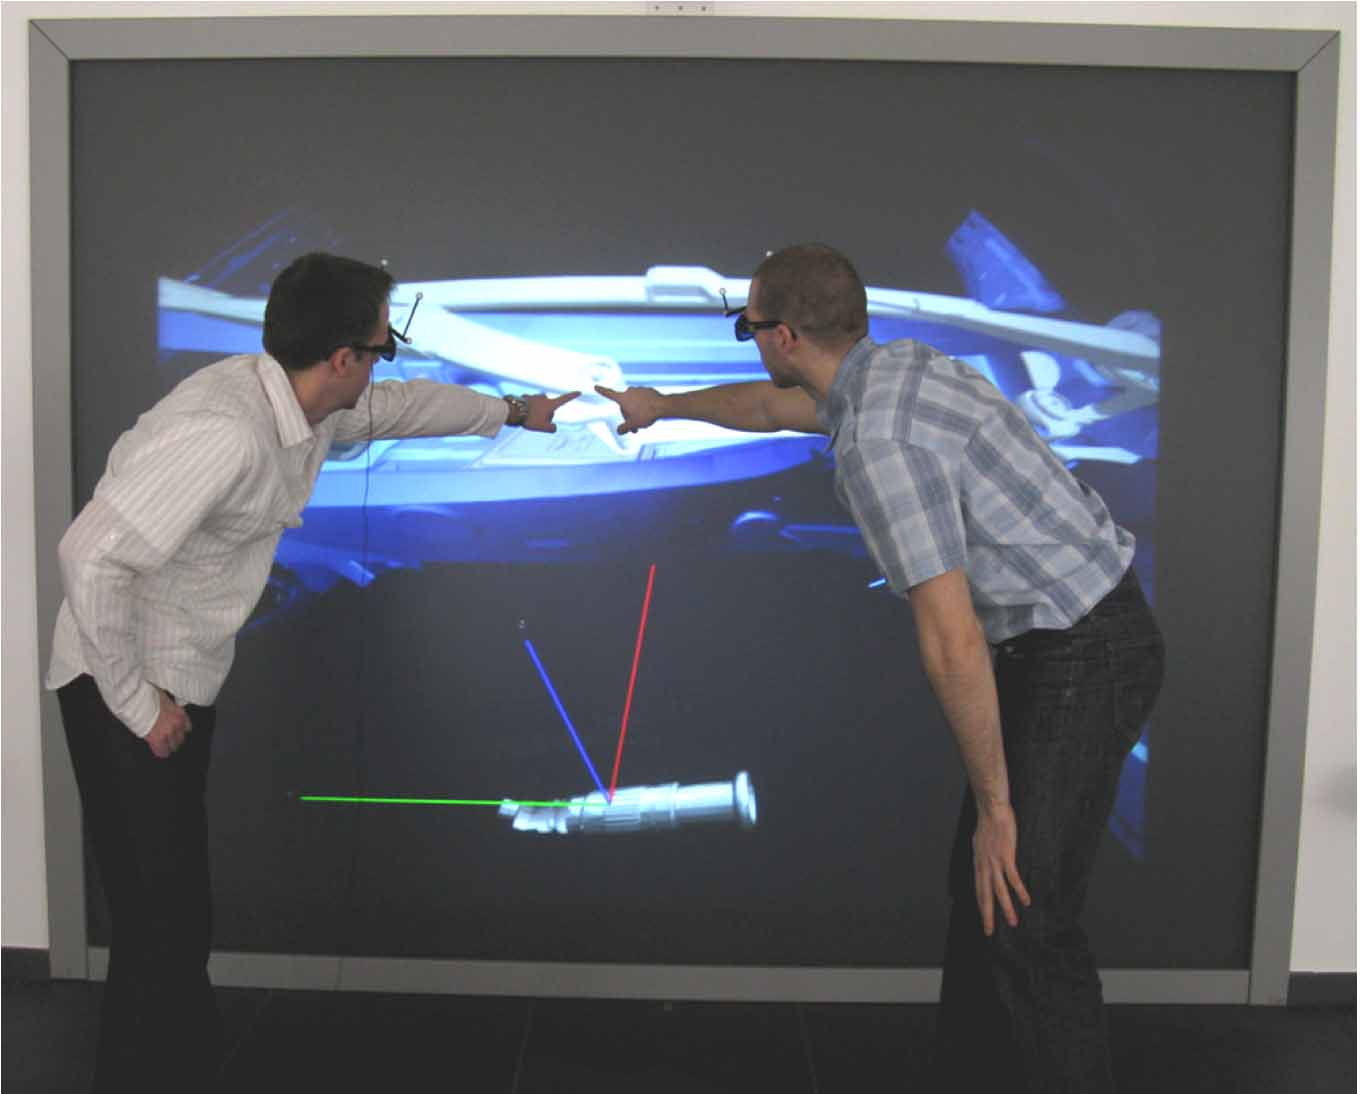
\includegraphics[width=\linewidth]{figures/ch2/pointing}
    \caption{Direct user interaction with deictic gestures.}
    \label{fig:2_consistent_collab:pointing}
  \end{subfigure}
  \begin{subfigure}{.7\textwidth}
    \centering
    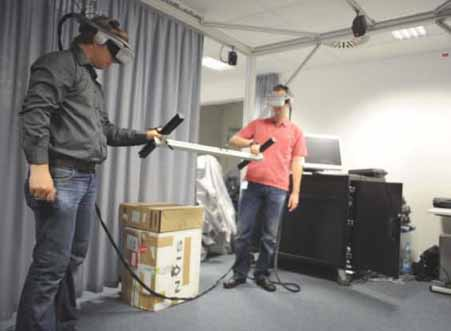
\includegraphics[height=4cm]{figures/ch2/tangible_1}
    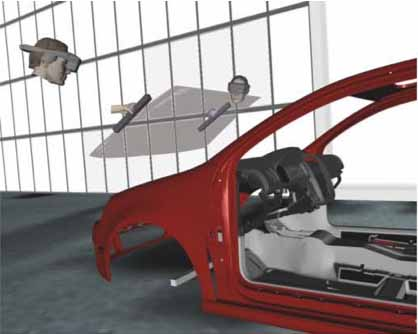
\includegraphics[height=4cm]{figures/ch2/tangible_2}
    \caption{A windshield assembly task using tangible interface.}
    \label{fig:2_consistent_collab:tangible}
  \end{subfigure}
  \begin{subfigure}{.45\textwidth}
    \centering
    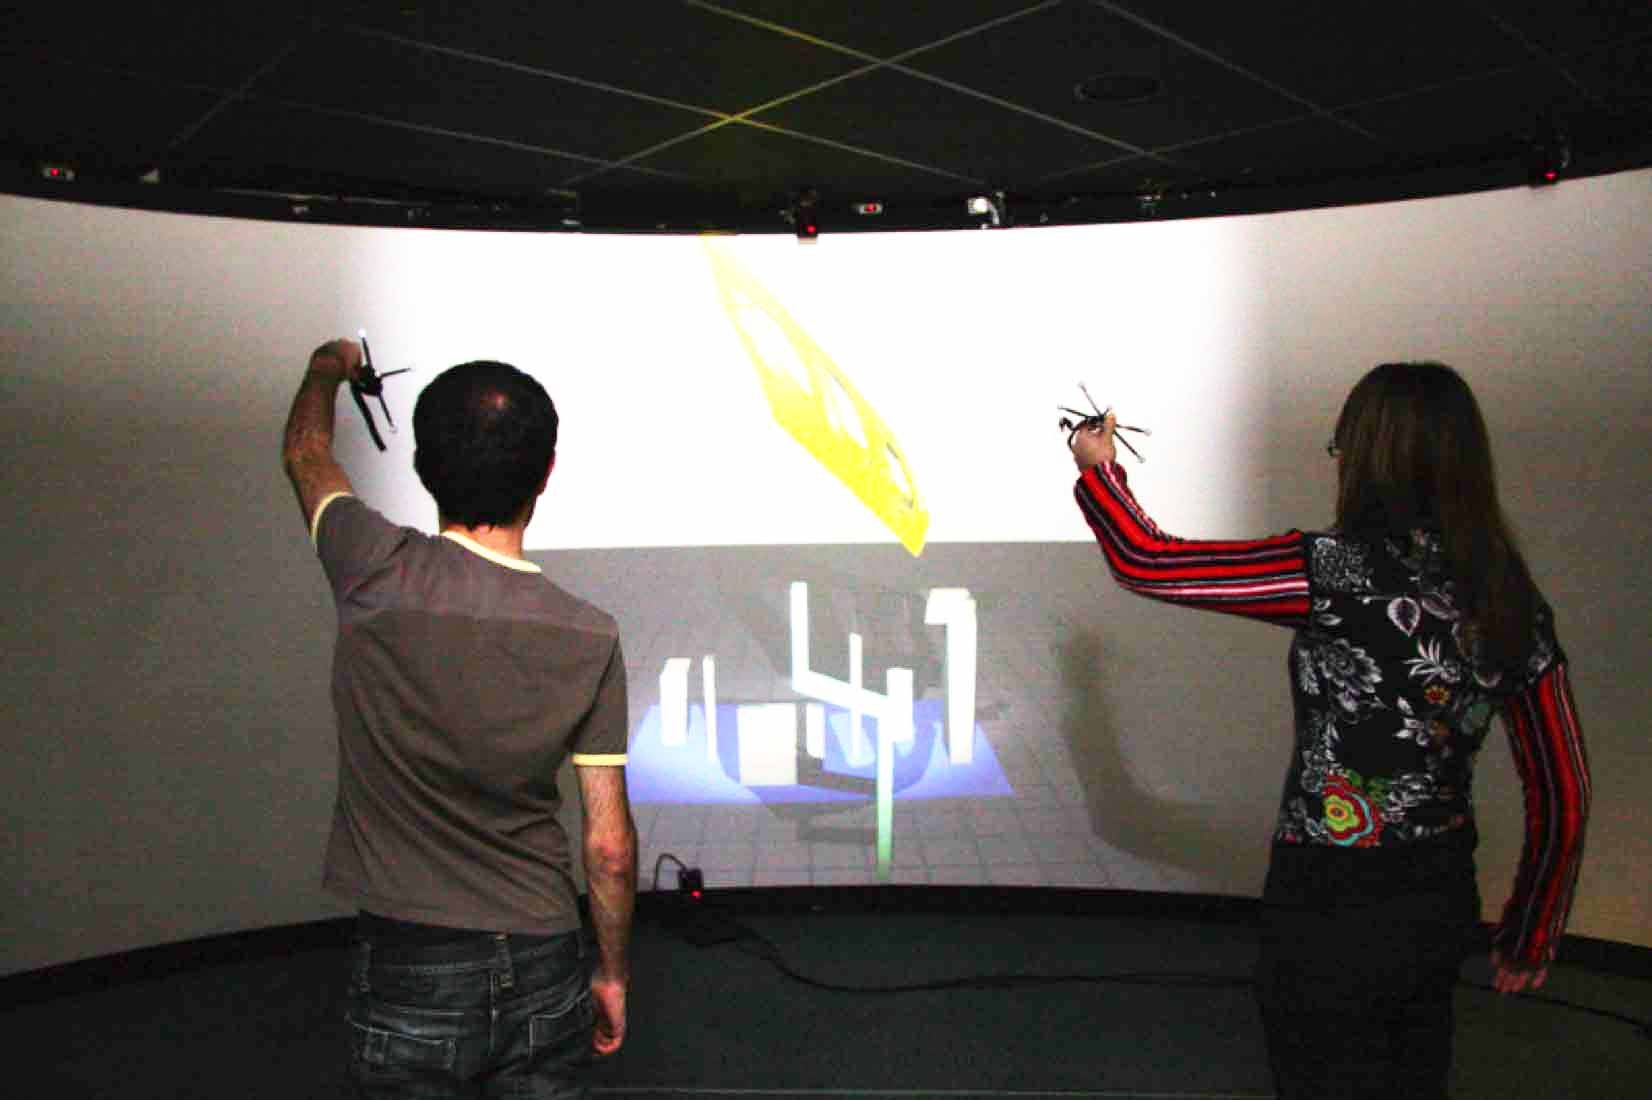
\includegraphics[height=4.6cm]{figures/ch2/comanip}
    \caption{Object co-manipulation with flysticks.}
    \label{fig:2_consistent_collab:comanip}
  \end{subfigure}
  \begin{subfigure}{.55\textwidth}
    \centering
    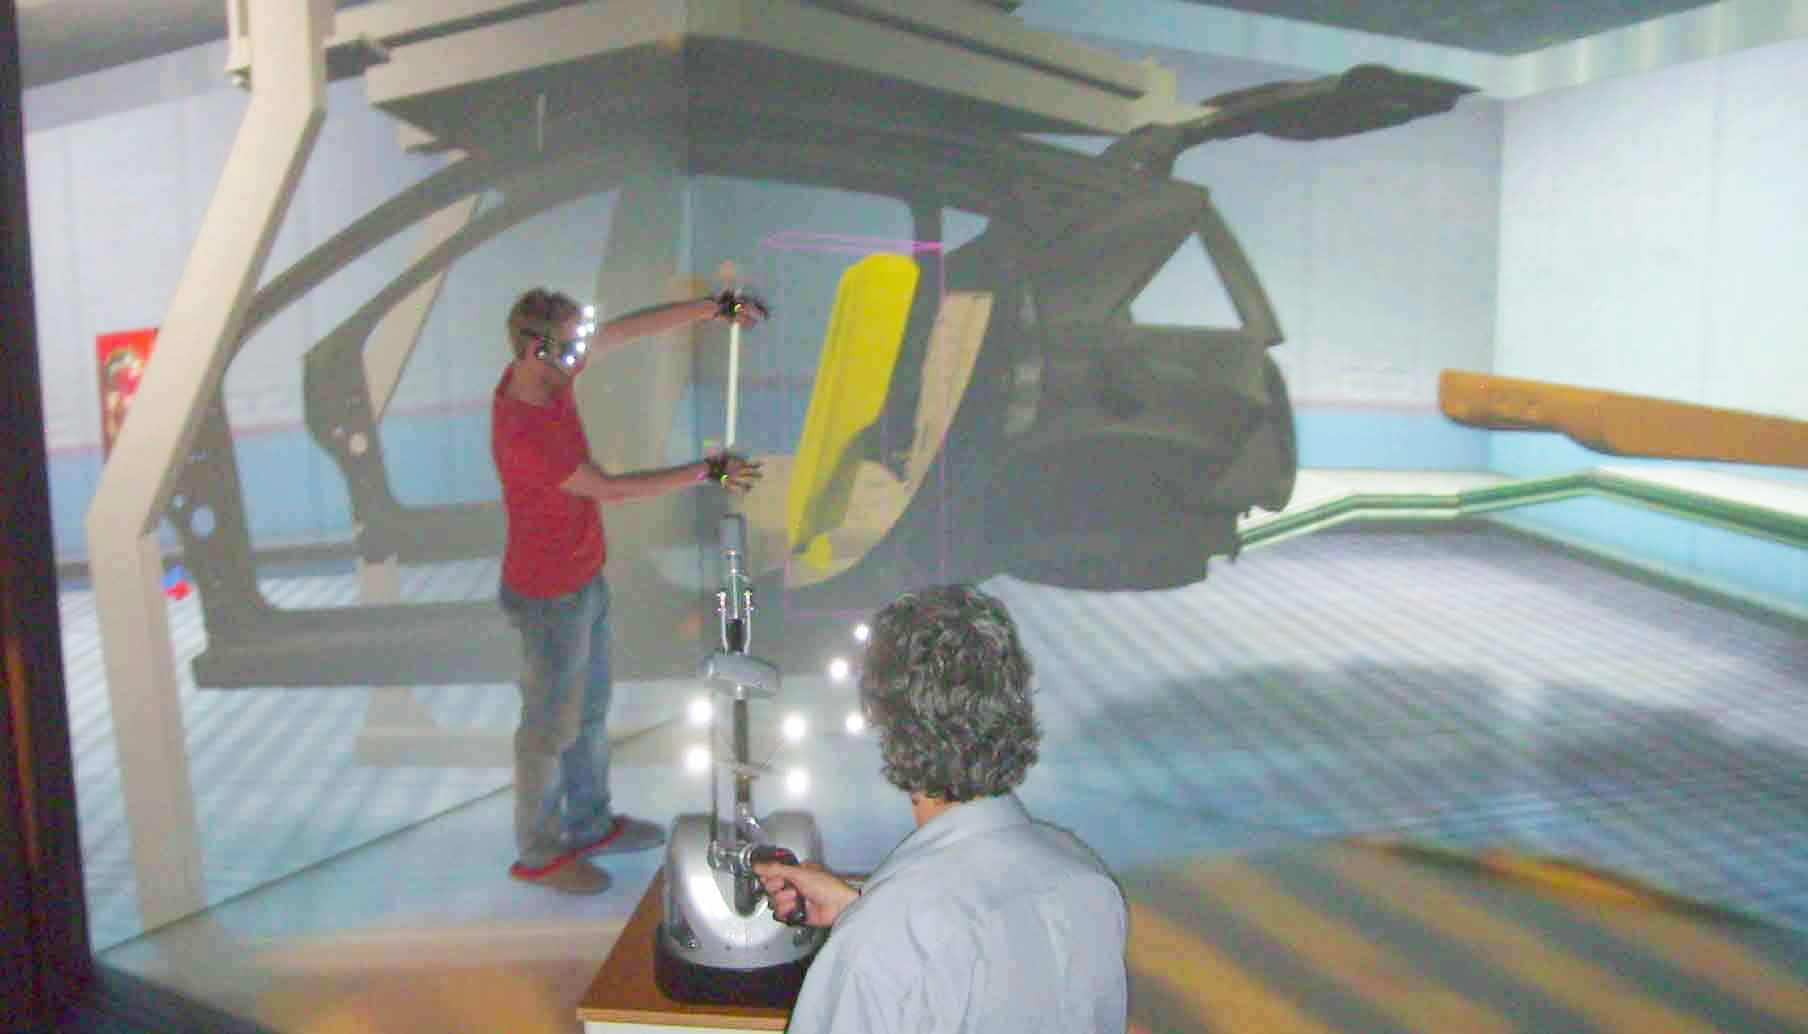
\includegraphics[height=4.6cm]{figures/ch2/malcomiics}
    \caption{MalCoMIICs demo for car assembly task.}
    \label{fig:2_consistent_collab:malcomiics}
  \end{subfigure}
  \caption{\label{fig:2_consistent_collab}Co-located collaborations in consistent mode.}
\end{figure}

The consistent mode is initially motivated by efforts to bring distortion-free stereoscopic view for each tracked user, and for a long time it is considered to be the default mode for co-located collaboration. This consistent mode suits well for closely-coupled collaborative tasks \citep{Simon2005First, Aguerreche2010Comparison, Martin2011Reconfigurable} (Figure~\ref{fig:2_consistent_collab:comanip} and \ref{fig:2_consistent_collab:malcomiics}) that do not require users to be or travel to different virtual places.

However, this spatial constrain restricts collaborative scenarios that can be supported in multi-user immersive virtual environment. Though several interaction techniques have been proposed to get around spatial constrains and to extend collaborative scenarios in consistent mode, such as the bent pick ray \citep{Riege2006Bent} and the see-through techniques \citep{Argelaguet2010STT}.

\paragraph{Individual Mode}
As opposite to consistent mode, the individual mode loosens constrains applied to users' spatial reference frames. This mode is complementary to the consistent mode and largely broadens collaborative scenarios that can be supported in the co-located use of immersive virtual environment. Collaborative scenarios can be extended in the following ways:

\begin{itemize}
\item Spatial distribution of users in the virtual world becomes more flexible:
\begin{itemize}
  \item Users are distributed at remote virtual places;
  \item Users are situated in a virtual space larger than the available physical workspace;
  \item Users are close to each other around an object of interest, but from different perspectives that they can get in consistent mode;
\end{itemize}
\item Artificial control of users' viewpoints:
\begin{itemize}
  \item To provide user with a third-person view or a god view of the virtual scene;
  \item To enable multi-scale observation (zoom on a particular zone);
  \item To quickly share one's first person view to others, or to exchange viewpoints between users \citep{Lopez2014Exchange}.
\end{itemize}
\end{itemize}

The individual mode can be very useful, even indispensable in some cases. For example, when two users working face-to-face in a projection-based immersive system, objects situated between them can not be correctly perceived since images on the screen are occluded by user's body. In this case individual mode can be applied to allow users to be virtually face-to-face while being side-by-side physically.

In fact, individual mode puts users in an intermediate state between remote collaboration through CVE where all interactions are mediated by the computer network, and consistent co-located collaboration where users can interact the same way as they do in the real world. In individual mode, the physical collocation still allows direct user communication in verbal and non-verbal form (e.g. one wants another to stop moving a table, he or she can simply say ``stop" or show a stop hand gesture). However, since users' spatial relationship (relative position and orientation) in the virtual world is no longer constrained by the one in the physical workspace, direct user interaction and communication involving spatial information may become confusing (e.g. the same virtual object will appear at different spatial locations for users who do not share the same spatial reference frame). In this case, embodied avatars as those used in remote situations are often needed to allow coherent user interactions.


\paragraph{Mode Switching}
Complex collaborative tasks often involve both shared and individual activities that require different spatial configurations of users, which could be identified as different coupling stages \citep{Lissermann2014PMC}. For example, in a virtual assembly task, a scenario could be that users first need to get parts of a model at different storehouses and then come back to the assembly area to put them together. This task contains first a loosely coupled collaboration stage (individual object-searching), followed by closely coupled interactions (the assembly work). 

Multi-user immersive virtual environments designed for co-located collaboration should support both consistent and individual collaborative modes to cover as more scenarios as possible, and also to integrate advanced viewpoint control that facilitate user communication and understanding of the situation.

There are different ways to switch between different collaborative modes by splitting or merging users' spatial reference frames that are summarized as follows:

\begin{itemize}
\item User initiated commands (e.g. button, gesture or vocal command, etc.);
\item Automatic transitions (i.e. embedded in the story line of the task);
\item Event-driven design (e.g. triggered when users enter or leave a certain zone in the virtual world).
\end{itemize}


\subsubsection{Virtual Navigation}
Navigation is a basic type of interaction for user to accomplish various tasks in the virtual world. A lot of navigation techniques of different nature exist to allow users to travel through large virtual space.


\paragraph{Navigation in IVE}
Navigation methods used in immersive virtual environments are in general different with desktop-based ones. At least two requirements should be met when designing navigation technique in such context:

\begin{itemize}
\item Desktop-based input devices like mouse and keyboard are not preferred as they are not compatible with behavioral interfaces;
\item Users should have access to an infinite virtual world while staying in a limited physical workspace.
\end{itemize}

Natural walking is considered to be the most intuitive way to explore the virtual environment \citep{Ruddle2009BW}. However, due to the limited size of available physical workspace, we need additional controls to enable infinite walking in restricted real workspace. Both hardware solutions like various locomotion devices (e.g. treadmills \citep{Iwata1999Treadmill}) and software solutions (e.g. redirection \citep{Peck2008RED}, resetting \citep{Williams2007ELV} and scaling techniques \citep{Interrante2007SLB}) are proposed to tackle the space limitation. Other metaphors like walk-in-place \citep{Razzaque2002RWP} and WIM (World-In-Miniature) \citep{Stoakley1995VRW} are also interesting alternatives.

Unlike previous techniques, rate control techniques activate virtual navigation by setting the velocity of user's spatial reference frame (we can imagine that the user is on board a virtual vehicle) instead of its position and orientation. Users can have the sensation of navigating (self-motion illusion or vection \citep{Riecke2012Vection}) without moving physically. Actually the virtual vehicle can be controlled by information coming from different sources, for example, various input devices like joystick, haptic arm \citep{Martin2012Forklift} or even specific locomotion devices \citep{Marchal2011JOYMAN}. With video cameras or optical tracking systems, users can specify the velocity of the vehicle by motion tracking data of the hand (camera-in-hand \citep{Ware1990EVC}) or head movements \citep{Bourdot2002HCNav}. Gestures \citep{Konrad2003Gesture} and postures \citep{Kapri2011Steering} can also be used to move the virtual vehicle. Bowman et al. named this kind of virtual navigation techniques steering metaphors \citep{Bowman2004UIT} which are often relatively easy to implement and can provide efficient and flexible control of virtual navigation.

Some navigation metaphors such as the bubble technique \citep{Dominjon2005Bubble} and the magic barrier tape \citep{Cirio2009MBT} combine both position and rate control in order to enable infinite navigation within restricted real workspace. Position control is used within the physical workspace and then rate control is applied to the virtual vehicle to move further in the virtual world. \citet{Cirio2012Cube} summarized several metaphors for safe navigation in a restricted cubic workspace. Moreover, \citet{Fleury2010Generic} proposed a general model to integrate physical workspace into the virtual world and make the user aware of the physical environment in different ways.

\paragraph{Navigation in Multi-user IVE}
In a multi-user immersive virtual environment, existing studies on co-located collaboration focused mainly on closely-coupled collaboration (e.g. co-manipulation) in consistent mode. In this situation, virtual navigation is often disabled. When users need to change the place for collaboration, navigation is conducted in a leader-follower mode that one user controls the navigation for the whole group. Spatial consistency is always maintained \citep{Beck2013IGG} (Figure~\ref{fig:2_group_navig:group_navig_1}) or temporarily disabled \citep{Kulik2011CSS} in certain cases to avoid virtual obstacles (Figure~\ref{fig:2_group_navig:group_navig_2}).

\begin{figure}[htb]
  \begin{subfigure}{.5\textwidth}
    \centering
    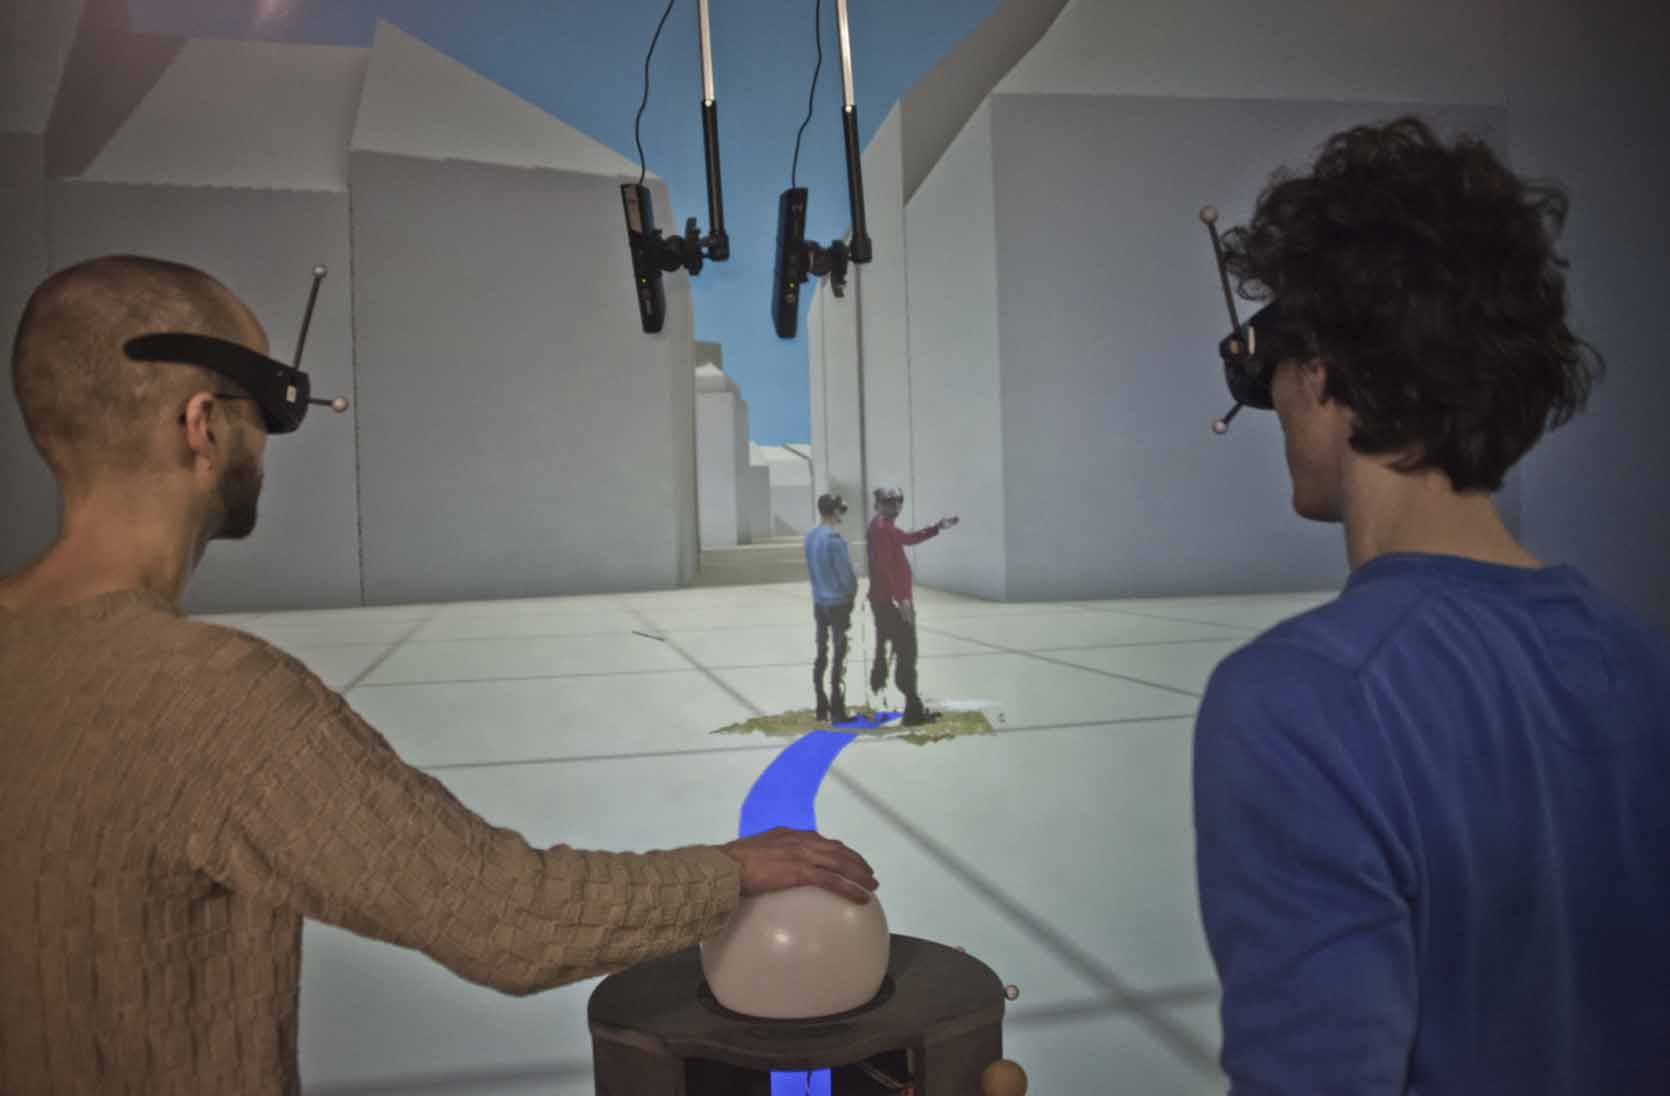
\includegraphics[height=5cm]{figures/ch2/group_navig_1}
    \caption{Group navigation controlled by the user on the left using a trackball.}
    \label{fig:2_group_navig:group_navig_1}
  \end{subfigure}
  \begin{subfigure}{.5\textwidth}
    \centering
    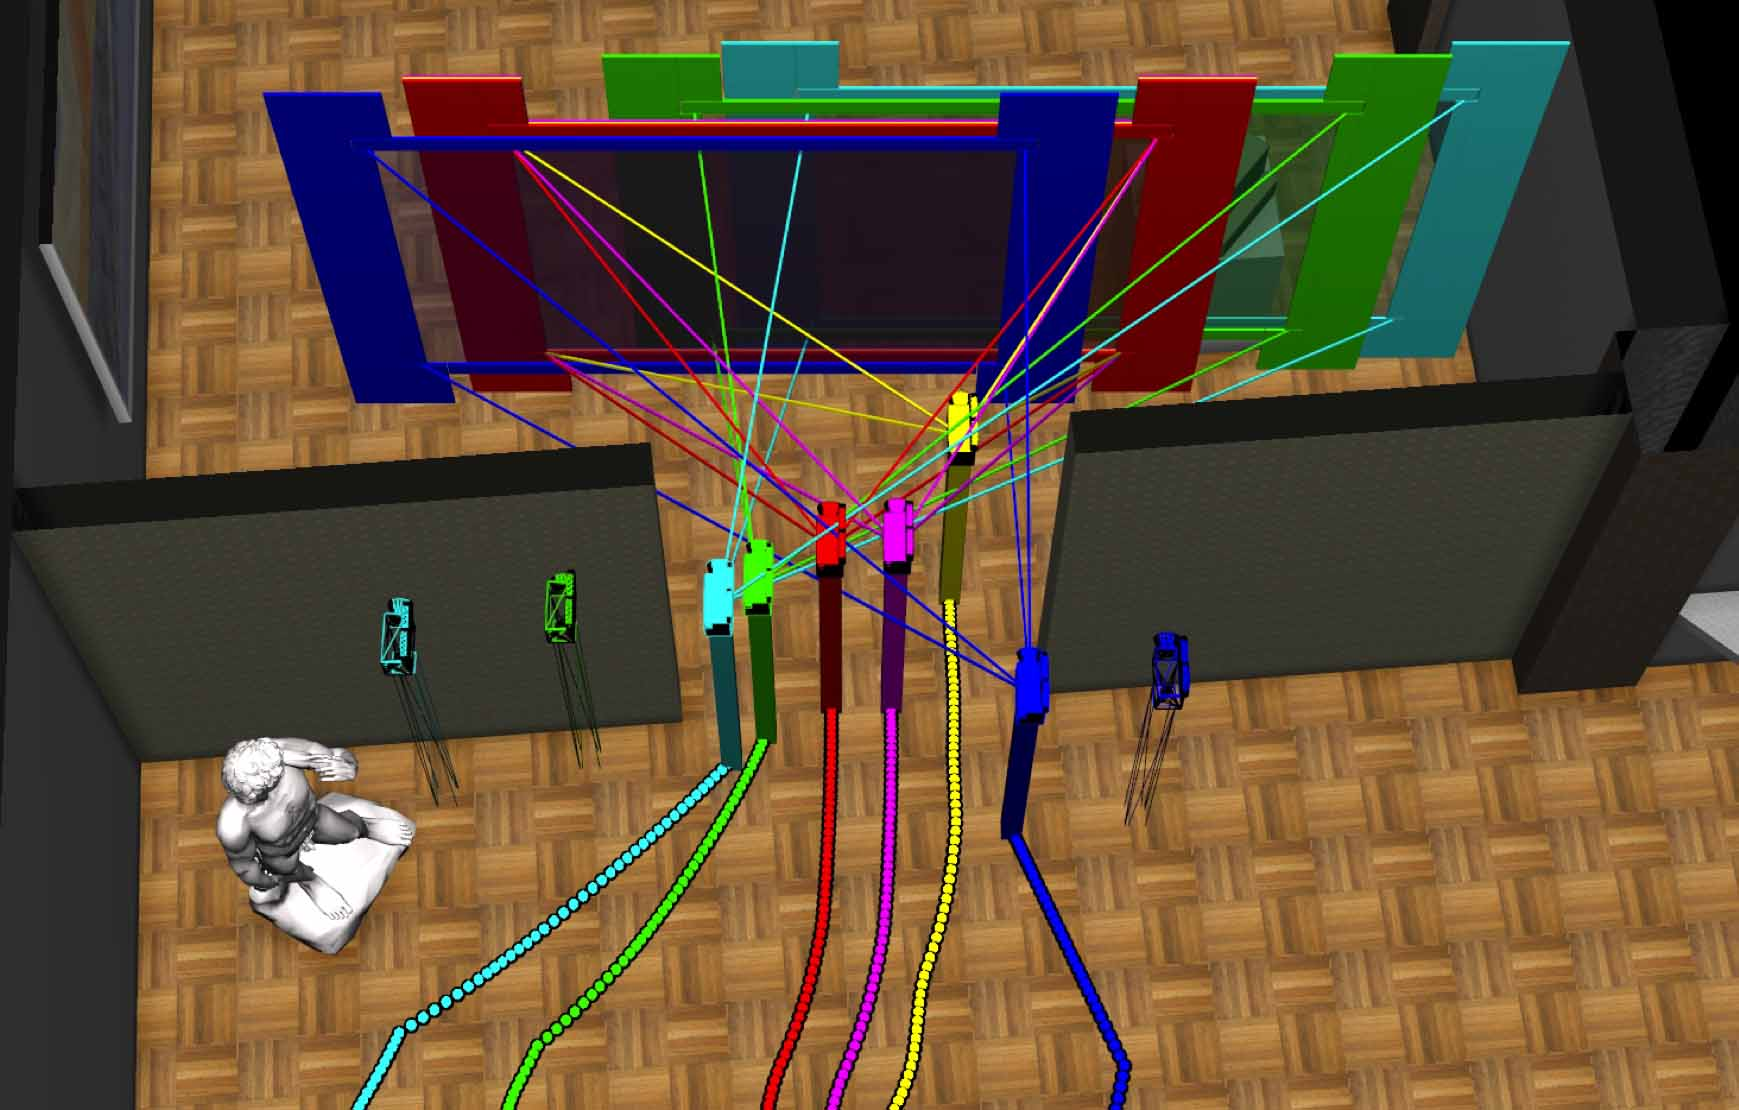
\includegraphics[height=5cm]{figures/ch2/group_navig_2}
    \caption{Users' viewing frustums are shifted towards the open passage to avoid passing through the wall.}
    \label{fig:2_group_navig:group_navig_2}
  \end{subfigure}
  \caption{\label{fig:2_group_navig}Navigation of co-located users controlled by a leader.}
\end{figure}

In individual mode, individual navigation can be easily achieved by providing independent navigation metaphors for each user which gives users full control on their own virtual locations. However, navigation metaphors based on users' physical movements may be problematic as users share the same physical workspace. Thus multi-user navigation models with individual navigation control should comply with user cohabitation constrains that will be discussed in the following section.


% -------------------------------------------------------------------------------------------------

\subsection{Addressed Issues}
As presented above, co-located collaboration in IVE contains two different collaborative modes: the consistent mode and individual mode. In consistent mode, users have a distribution of virtual spaces that are coherent with their physical workspace, which offers a similar interaction experience as in real world. On the contrary, users in individual mode have independent viewpoints which broadens supported collaborative scenarios with more flexible viewpoint control.

However, due to the inconsistency between users' spatial distributions in the virtual world and real workspace, the individual mode provides users with a new kind of perceptual immersion and related cognitive experiences as they need to handle information from both real world and the virtual scene at the same time. We identified two main categories of spatial issues: perceptual conflicts during user communication and interaction, and user cohabitation in limited physical workspace. These issues should be studied if we want to validate the use of individual mode for co-located collaboration in IVEs. 


\subsubsection{Perceptual Conflicts}
Communications between collaborators are usually conducted in a multimodal way \citep{Paggio2005Multimodal} including verbal and non-verbal modalities \citep{Ennis2010Seeing, Dodds2011Talk}, especially deictic gestures to refer to objects or places. In individual mode, this kind of spatial interactions can be restored by introducing embodied avatars just like in remote situations - each user interacts temporally with other users' avatars instead of the real user in his/her own ``copy" of virtual world.  As a consequence, multimodal interactions in individual mode lead to two kinds of perceptual conflicts:

First, in projection-based immersive systems, users sharing the same display may sometimes enter each other's field of view when they work with embodied avatars. The simultaneous perception of a user and his/her avatar leads to a special experience that we called ``dual-presence". The dual-presence offers conflicting visual cues because the perceived real user and corresponding avatar share some common properties in terms of appearance and body movement (animated by real-time motion capture).

For example, in a two-user collaborative scenario (Figure~\ref{fig:2_pc_dualpresence}), user A is pointing at a cube next to him/her for user B to delete it. User B may be troubled by seeing both the real user A and his/her avatar doing the pointing gesture, and it may be more confusing when there happens to be another virtual object (e.g. a cylinder) in the pointing direction of real user A.

\begin{figure}[htb]
  \centering
  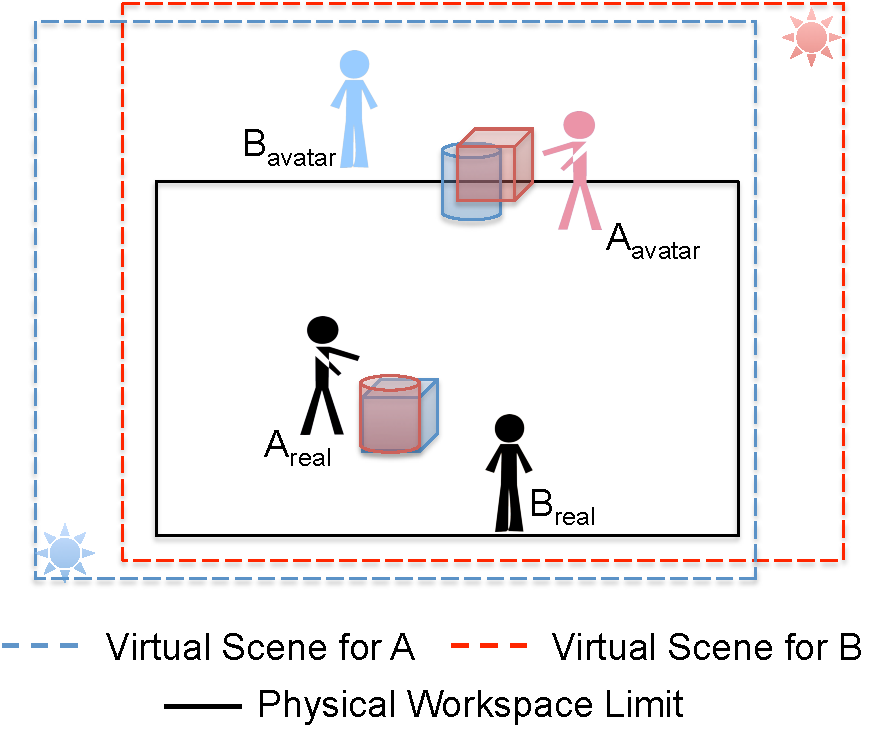
\includegraphics[width=.7\textwidth]{figures/ch2/pc_dualpresence}
  \caption{\label{fig:2_pc_dualpresence}Illustration of dual presence with a two-user scenario, two users are virtually face-to-face while standing side-by-side. User B simultaneously perceives that the real user A and A's avatar is pointing at different virtual objects.}
\end{figure}

Second, in individual mode, users dialogue with each other while interacting via embodied avatars. Since co-located users talk to each other directly without computer mediation, hearing someone from a different location than his/her visual representation (i.e. avatar) results in a visual-auditive conflict. Still in a two-user example (Figure~\ref{fig:2_pc_visualauditive}), user B is looking at user A's avatar in front, but the audio source (i.e. real user A) is on his/her left.

\begin{figure}[htb]
  \centering
  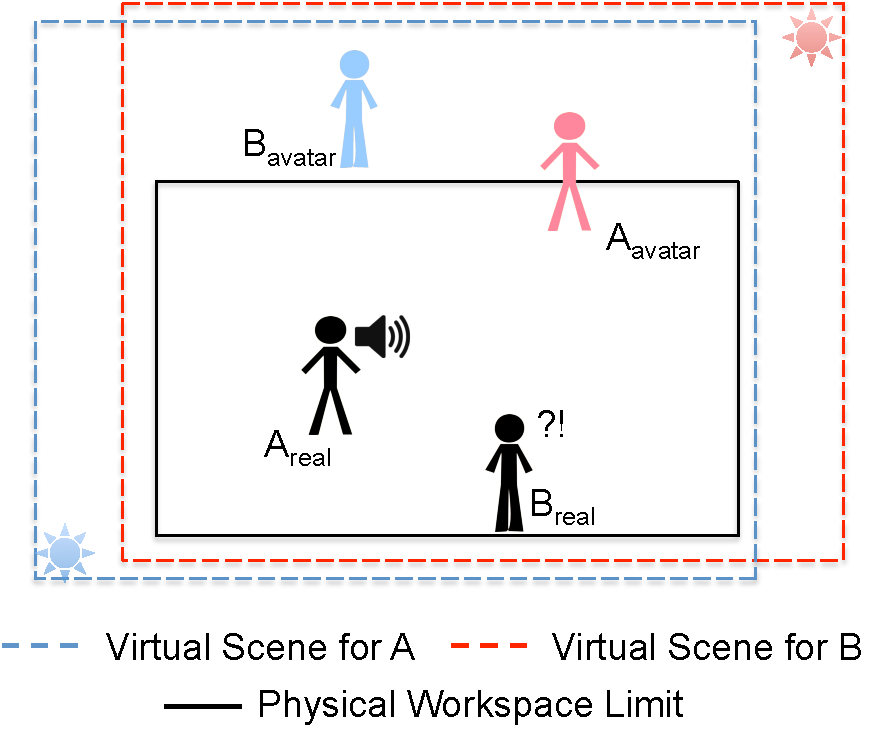
\includegraphics[width=.7\textwidth]{figures/ch2/pc_visualauditive}
  \caption{\label{fig:2_pc_visualauditive}Illustration of visual-auditive conflicts with a two-user scenario. User B experiences visual-auditive spatial conflicts when focusing on user A's avatar in front while talking to the real user A situated at a different location.}
\end{figure}

Although according to \citet{Spence2013Just}'s review, spatial coincidence does not represent a general constraint on multi-sensory integration in humans, but would be a much more task-dependent phenomenon. However, in a multi-user IVE, this visual-auditive conflict could be amplified due to the flexibility of virtual environment. For example, users could be far away from each other in the virtual world and they still hear each other from a close distance.

These two categories of perceptual conflicts are interrelated since they all depend on the distance between a user and his/her avatar. We need to study the usability of individual mode for co-located collaboration by investigating users' reaction to dual-presence and visual-auditive conflicts. The effects of such perceptual conflicts will influence choices on the design of co-located collaborative immersive systems. For example, whether we should prevent users from seeing the real users to avoid dual-presence, whether we need headphones to map users' speech to avatars' positions by 3D audio, etc.


\subsubsection{User Cohabitation}
Users in a multi-user IVE are subjected to two kinds of spatial constrains: users are inside a limited physical workspace, and they share the same workspace. These two constrains lead to different aspects of user cohabitation management: how to manage the spatial relationship between active users and the workspace boundaries while keeping good visual immersion? How to allocate personal workspace for users so that they won't collide or occlude each other?

Immersive virtual environment has the power to bring users to an artificial world by blocking the perception of the real world. In such situation users often forget boundaries of the physical workspace due to visual immersion, so when they move around in such system they risk to run into walls (with HMDs) or screens (projection-based display) which could endanger both the user and the device. Moreover, visual immersion is limited by functional tracking area and the screen configuration (for projection-based display). For example, in large projection-based immersive systems with non-closed displays such as large image wall or a 3-wall CAVE, visual immersion is limited to the display area (Figure~\ref{fig:2_illu_system}).

\begin{figure}[htb]
  \centering
  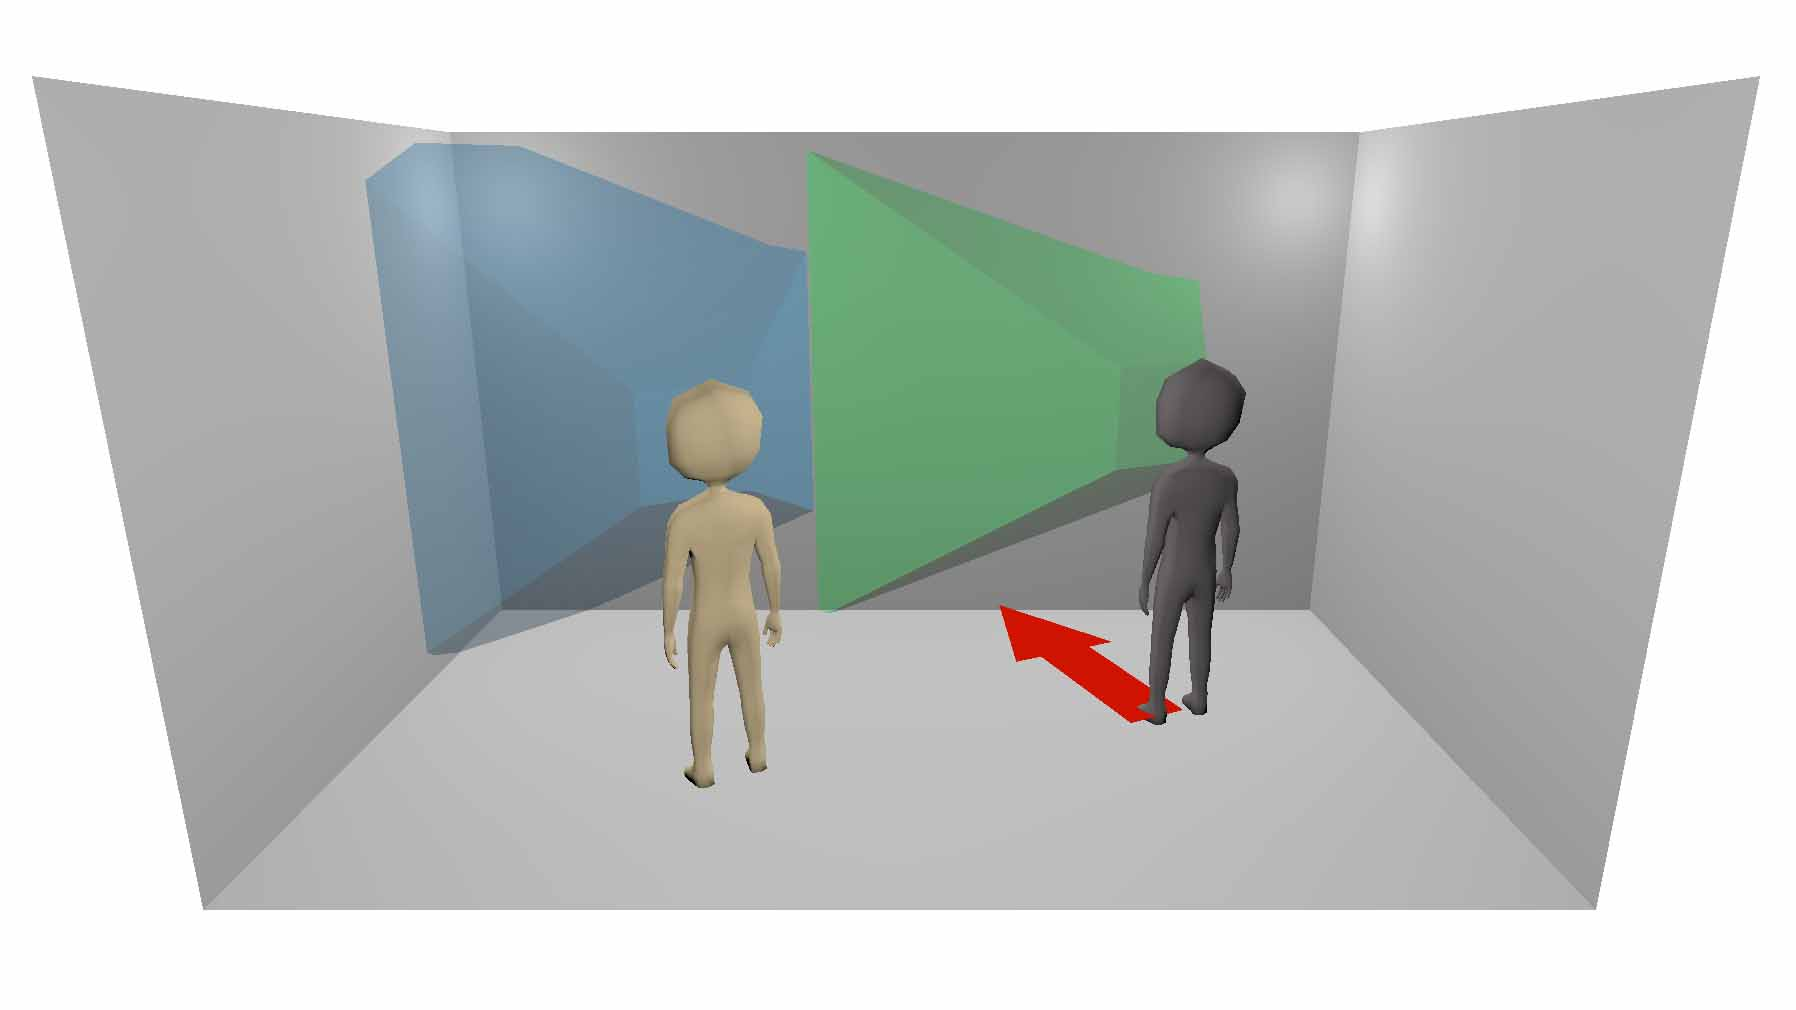
\includegraphics[width=0.49\textwidth]{figures/ch2/illu_wall_col}
  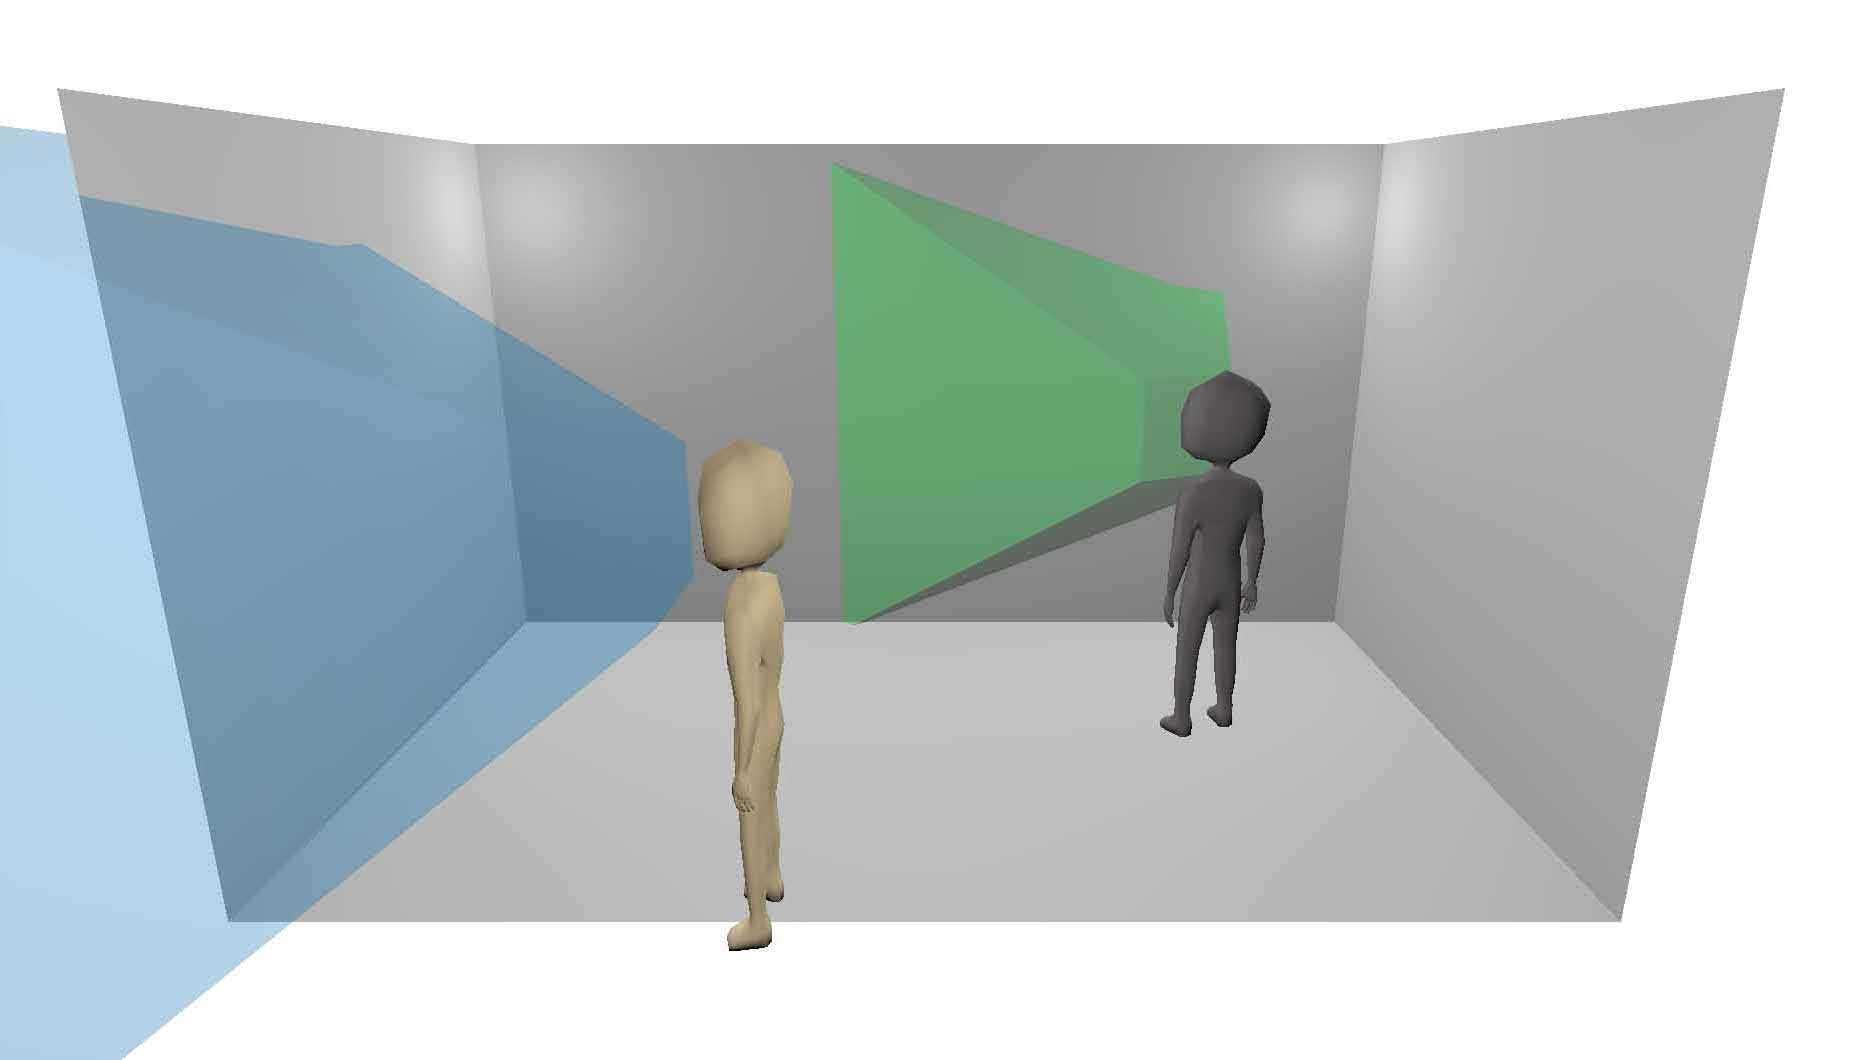
\includegraphics[width=0.49\textwidth]{figures/ch2/illu_empty}
  \caption{\label{fig:2_illu_system}Illustration of workspace boundary for translation (left) and looking direction (right) in a multi-stereoscopic 3-wall CAVE.}
\end{figure}

\begin{figure}[htb]
  \centering
  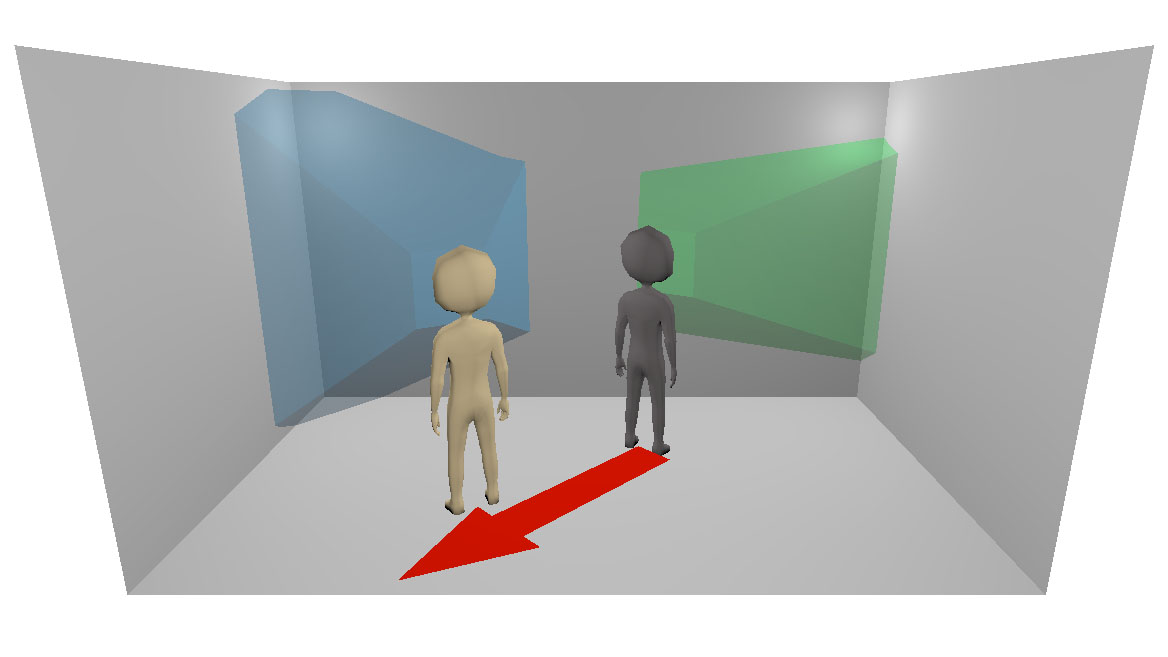
\includegraphics[width=0.49\textwidth]{figures/ch2/illu_user_col}
  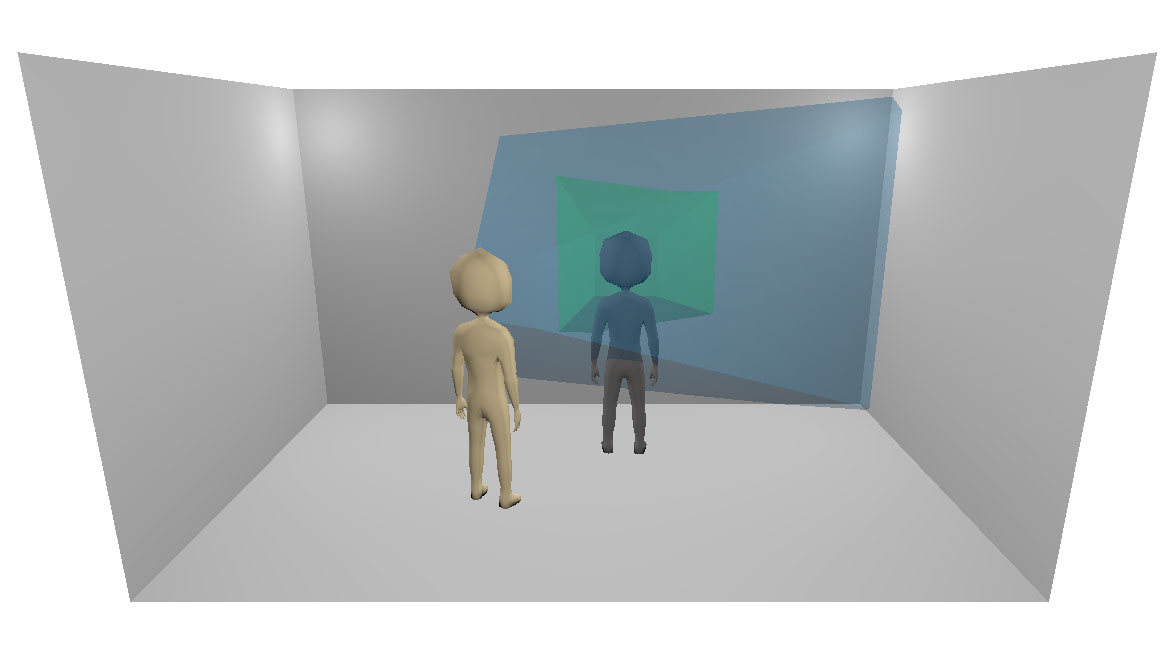
\includegraphics[width=0.49\textwidth]{figures/ch2/illu_occ}
  \caption{\label{fig:2_illu_users}Illustration of collision (left) and occlusion (right) between co-located users in a multi-stereoscopic 3-wall CAVE.}
\end{figure}

When multiple users share the same immersive device for co-located collaboration in individual mode, they may run into collision when they move around without paying attention to the others. In projection-based immersive systems, one's visual perception of the virtual world could be disrupted by another if the latter appears to be in the field of view of that user due to body occlusion (Figure~\ref{fig:2_illu_users}).

Depending on the choice of display technology and screen configuration, not all aforementioned issues are present in all types of immersive systems. Here Table~\ref{tab:cohab_issues} divides all cohabitation issues into different categories: some are inherent issues of the individual collaborative mode, others are more system-dependent, i.e. depending on the type and configuration of used immersive display. For example, user occlusion merely appears in projection-based immersive system, and perceiving ``empty screen" is only possible with non-closed immersive display. 

\begin{table}[htb]
\renewcommand{\arraystretch}{1.3}
\caption{Cohabitation Issues in Multi-user Immersive Systems.}
\label{tab:cohab_issues}
\centering
\begin{tabular}{l l l}
  \hline
   & Workspace-related & User-related \\ \hline
  Generic & Collision with workspace border & Collision between users \\
  System-dependent & Seeing non-projected area & User occlusion \\ \hline
\end{tabular}
\end{table}

For safe and efficient use of multi-user IVEs, new paradigms are needed to enable individual navigation in infinite virtual space while keeping users' level of immersion and safety.

% -------------------------------------------------------------------------------------------------


\subsection{Approach}
To assess users' reactions to certain stimuli (e.g. perceptual conflicts) or the performance of novel paradigms (e.g. paradigms for navigation or object manipulation) in virtual environments, experiment-based user evaluation inherited from HCI research has become a mainstream method. Besides formative user experiment, there are many other evaluation methods such as cognitive walkthrough, heuristic expert evaluation, interview, post-hoc questionnaire and so on, each can help us to gather some information from a different angle with certain cost \citep{Bowman2002Survey}.

In the context of this thesis, our goal is to study spatial issues related to individual collaborative mode in order to design a valid and efficient framework for co-located collaboration in IVE. Experiments below are conducted in projection-based immersive system in which all spatial issues that we mentioned are present. The main experimental platform named EVE (Evolutive Virtual Environment), is a four-screen multi-user immersive CAVE system built with the active \& passive separation technique (see Appendix~\ref{appendix:platform}). It serves as an experimental tool to study issues related to user interaction and communication for co-located collaboration in projection-based multi-user immersive virtual environment.

The first step is to study effects and influencing factors of perceptual conflicts due to the introduced avatar representation for co-located collaboration. We want to examine how perceptual conflicts generated by dual-presence would alter users' communication and their task performance. In a two-user case study, participants receive instructions from an experimenter to accomplish an object-picking task, we artificially created different levels of perceptual conflicts by varying the distance between the real experimenter and her avatar, and also by changing modalities involved in the instructions (verbal and/or gestural). A post-hoc questionnaire was designed to collect users' subjective feelings towards dual-presence and their understanding of the instructions. This experiment is presented in detail in Chapter~\ref{chapter:expe_perception}.

Second, we concentrate on the design and evaluation of appropriate navigation paradigms to allow individual navigation while solving user cohabitation problems in a progressive way. The paradigm that we propose is based on a Human Joystick metaphor controlled by head tracking \citep{Bourdot2002HCNav}. First we evaluated this metaphor by a comparative experiment \citep{Chen2013NVW} to confirm its advantages over traditional navigation solutions (e.g. joystick). Then we created an Altered Human Joystick paradigm by adding additional controls to manage users' relationship with system borders and to minimize inter-user interferences.

Chapter~\ref{chapter:expe_cohab} presents the implementation of Altered Human Joystick along with metrics that we defined to evaluate cohabitation capacity in response to identified cohabitation problems. A series of experiments were carried out to test different alterations to see their influences on user distribution and to find an optimal combination.

At last, in Chapter~\ref{chapter:kinematic_model}, we designed a kinematic model which integrates real world information into the virtual navigation control in the aim of providing a general framework for co-located collaboration by supporting both consistent and individual modes and also fluent transition between them.


\section{Chapter Summary}
The research described in this thesis consists of investigating how to enable individual mode to better support co-located collaboration in multi-user IVEs. The first part of this chapter outlines motivations and techniques to create immersive systems for co-located collaboration. Then the second part presents notions and issues related to spatial aspects of co-located use of IVE, it also summarizes research efforts that we made to study these issues and to propose solutions accordingly.

To fully support co-located collaboration in multi-user IVE, our approach is to study and to resolve separately the spatial issues that we identified in the aim of building a general framework for co-located collaboration in IVE which allows both consistent and individual modes.